\documentclass{main}

\usepackage[table,xcdraw]{xcolor}
    

\usepackage{graphicx}      % include this line if your document contains figures
\usepackage{natbib}        % required for bibliography
\usepackage{enumerate}
\usepackage[utf8]{inputenc}
\usepackage{float}
\usepackage[centerlast,small,sc]{caption} 
\setlength{\captionmargin}{30pt}
\usepackage[none]{hyphenat} 
\usepackage{subcaption} 
\usepackage{capt-of}
\usepackage{kpfonts}
\usepackage{calc}
\usepackage{hyperref}
\newlength\shlength
\newcommand\xshlongvec[2][0]{\setlength\shlength{#1pt}%
  \stackengine{-5.6pt}{$#2$}{\smash{$\kern\shlength%
    \stackengine{7.55pt}{$\mathchar"017E$}%
      {\rule{\widthof{$#2$}}{.57pt}\kern.4pt}{O}{r}{F}{F}{L}\kern-\shlength$}}%
      {O}{c}{F}{T}{S}}
\sloppy  
\newcommand{\specialcell}[2][c]{%
  \begin{tabular}[#1]{@{}c@{}}#2\end{tabular}}
  
\begin{document}

\begin{frontmatter}

\title{State of the art of robotic solutions for \textit{in situ} hard coating
of hydraulic turbines\thanksref{footnoteinfo}} 

%TODO Verificar contrato ESBR
\thanks[footnoteinfo]{This work is supported by ESBR under contract COPPETEC
JIRAU 09/15 6631-0003/2015 (ANEEL R\&D program).}

\author[1]{Eduardo Elael M. S.}
\author[1]{Estevão F. Ferrão} 
\author[1]{Gabriel Alcantara C. S.}
\author[1]{Ramon R. Costa}
\author[1]{Renan S. Freitas}

\address[1]{Department of Electrical Engineering, COPPE UFRJ, Rio de Janeiro, Brasil} 
  
\begin{abstract}                % Abstract of not more than 250 words.
%TODO Renan: Resumo
\end{abstract} 
 
\begin{keyword}
%TODO Renan: Keywords
\end{keyword}

\end{frontmatter}

\section{Introduction}

%%%%%%%%%%%%

The importance of regular maintenance on hydraulic turbines have already been
established (ref EMMA-SOTA), given that its power output have a near 46\%
increase after maintenance. Providing a meaningful gain for highly dependent
countries like Brasil and Norway.

% Em EMMA-SOTA, é apresentada a importância da manutenção regular das turbinas em
% uma usina hidrelétrica, já que, em sua operação ideal e de máxima eficiência,
% sua potência tem aumento de quase 46\% após manutenção. Aumento significativo,
% principalmente para países dependentes desta forma de energia, como o Brasil e
% Noruega.

The efficiency of a hydraulic turbine is related at some extend to the hydraulic
profile of the runner blades and its degradation is mainly due to two
phenomena: cavitation and abrasion. As a protective measure, the blades are
hardcoated by a process called HVOF (High velocity oxy-fuel coating spraying),
which mitigate the damage caused by the aforementioned effects, but has to be
reapplied periodically.

The hardcoating process can take up to two months per turbine, including turbine
disassemble, blade's hardcoating on a specifically designed environment and
following remounting and calibration.

% A eficiência de uma turbina hidrelétrica depende de inúmeras variáveis, como
% volume de água, queda d'água, o tipo da turbina, o distribuidor e outras. O
% projeto EMMA tem foco na manutenção do perfil hidráulico das pás dos rotores de
% turbinas hidrelétricas, por este se degradar com maior rapidez, exigindo
% manutenções recorrentes. 

% A fim de proteger a pá contra abrasão e cavitação é realizado processo de
% revestimento por asperção térmica, ou, especificamente, a metalização (HVOF).
% Atualmente, este processo pode levar cerca de dois meses por turbina,
% já que exige que a turbina seja desmontada, as pás serem processadas em
% outro ambiente, a turbina seja remontada e recalibrada.

Aiming to reduce the downtime assossiated for the hardcoating process, robotic
\textit{in situ} solutions, i.e. inside the runner environemnt, consisting of a
insdustrial robotic arm mounted over a customized base are scrutinized. This is
the main objetive of the EMMA project, a R\&D project by Fundação Coordenação
de Projetos, Pesquisas e Estudos Tecnológicos (COPPETEC), in partnership with
Rijeza company, Agência Nacional de Energia Elétrica (ANEEL) and Energia
Sustentável do Brasil (ESBR).

Despite the generic approach of this article, the bulb turbine facilities are
different for each power plant. The reference hydroeletric power plant for the
ideas discussed here is the UHE Jirau, near Porto Velho(Brazil - RO). The
Madeira river, where the UHE Jirau is located, has a high concentration of
suspended particles which entails further abrasion on the blades, it also has a
low water level diference of 2 to 20 meter intensifing cavitation. For more
details on the UHE Jirau please reference (EMMA SOTA), however it is important
to recall that there are two main entry points for runner area: the top hatch
with a 35.7 cm diameter, just above the turbine, and the bottom hatch with a 80
cm diameter on the draft tube, 10 m away from the runner and with a 4m access
duct from exterior ground level. But, as a top hatch is not a standard across
other hydroeletric power plants, e.g. the UHE de Santo Antônio near UHE Jirau,
the solutions focus on the bottom hatch.

The workflow for the \textit{in situ} hardcoating can be thought as a
sequence of 4 minor jobs:
Enter the runner area with the robot; Move the robot and anchor it in some
suitable positions near the blade to be hardcoated; Calibrate the robot, in the
sense of identifying the relative positions of the robot, blade and the rest of
the environment; And finally, check if the the robot's arm can cover the whole
blade.

The following sections explore the developments on the EMMA project, they are
organized so to mimic the workflow:
section 2 exposes the ideas for the customized base and related logistics;
section 3 describes the calibration process which has to be done once the robot
is well placed, but before it's able to start coating; section 4 explore the
robot arm's limitations for performing the hardcoating; And lastly section 5
concludes and discusses the future steps for the EMMA project.

% Apesar de o projeto visar uma solução genérica para turbinas bulbo, as
% instalações são diferentes em cada usina. Desta forma, o ambiente de testes
% deste projeto é a Usina Hidrelétrica de Jirau, localizada no Rio Madeira. O Rio
% Madeira carrega muitos sedimentos provocando maior abrasão nas pás, se comparado
% com outros usinas, além disso, a queda d'água de 2 a 20 metros intensifica o
% fenômeno de cavitação. As principais características das instalações da turbina
% em análise estão descritas em EMMA-SOTA, mas vale ressaltar a particularidade
% dos dois acessos principais ao aro câmara, relevantes para a busca de uma
% solução: acesso superior (35.7 cm de diâmetro) e acesso inferior (80 cm de
% diâmetro).

% O projeto EMMA busca uma solução para o processo de metalização \textit{in
% situ}, isto é, revestimento das pás no ambiente da turbina, diminuindo o tempo
% de manutenção e, consequentemente, de máquina parada.  A solução conceitual
% desenvolvida em EMMA-SOTA é a utilização de um manipulador industrial sobre uma
% base. As características do manipulador e da base variam de acordo com o
% acesso: no caso da escotilha superior, a solução é um manipulador industrial de
% pequeno porte e base customizada operada eletronicamente; no caso da escotilha
% inferior, a solução é um manipulador industrial de porte médio e base tipo
% trilho com acopladores magnéticos.
% 
% A análise das instalações da Usina Hidrelétrica de Santo Antônio, em Porto
% Velho, vizinha à Jirau, mostrou que as turbinas não possuem um acesso superior.
% A fim de tentar construir uma solução mais geral, o presente documento visa dar
% continuidade ao projeto, detalhando o estudo de viabilidade técnica para a
% solução da escotilha inferior.

%%%%%%%%%%%%%%%%%%%%%%%%%%%%%%%%%%%%%%%%%%%%%%%%%%%%%%%%%%%%%%%%%%%%%%%%%%%%
% According to the world energy council, hydropower is the most flexible and
% consistent of the renewable energy resources and, at the end of 2008, the total
% capacity of hydropower resources was 874 GW. Brazil is the second
% country in hydropower production, and second with the highest
% consumption of hydropower with a 70.000 MW installed capacity, and 433
% hydroelectric plants in operation. Since Brazil is one of the world's richest
% countries in water resources, and the hydropower is the most dominant across
% the country, it motivates the development and investment in hydropower
% generation., and Brazil is the .
% %\begin{figure}[h!]
% %	\includegraphics[width=\columnwidth]{figs/intro/graph.png}
% %	\caption{Top hydropower producing countries}
% %	\label{fig::cavitacao}
% %\end{figure}
% 
% %O Brasil é um dos países mais ricos do mundo em recursos hídricos, facilitando
% % o desenvolvimento e investimento em geração de energia a partir desse recurso. A
% %energia hidráulica é a mais dominante em todo o país, e o Brasil é o segundo
% %país com maior consumo de energia hidrelétrica no mundo com capacidade
% %instalada de 70.000 MW, 433 usinas hidrelétricas em operação. 
% 
% In Brazil, the renovation and improvement of the built large plants is estimated
% to result in a potential increase of 32.000 MW \citep{goldemberg2007energia}, a
% figure that can be achieved, in large part, by the maintenance of the
% hydropower turbines. These turbines are constantly exposed to abrasion and
% cavitation phenomena, which determine its life cycle.
% %Estima-se que a reforma e melhoria das grandes usinas construídas resultariam
% %em um aumento potencial de 32.000 MW \citep{goldemberg2007energia},
% %número que pode ser alcançado, em grande parte, pela manutenção das turbinas
% %geradoras da energia elétrica. As turbinas estão constantemente expostas aos
% %fenômenos de abrasão e cavitação, os quais determinam sua vida útil.
% 
% The cavitation phenomenon is very well studied and detailed in
% \cite{escaler2006detection}, which outlines their types, occurrences and
% effects in the different hydraulic turbines. This physical phenomenon can cause
% erosions in the hydraulic turbines, leading to water flow instability,
% excessive vibrations and turbine efficiency reduction.
% %O fenômeno de cavitação está muito bem estudado e detalhado em
% %\cite{escaler2006detection}, onde são apresentadas seus tipos, ocorrências e os
% %efeitos nas diferentes turbinas. Esse fenômeno físico pode causar erosões na
% %máquina hidráulica (figura~\ref{fig::cavitacao}), gerando instabilidade de
% % fluxo de água, vibrações excessivas e redução da eficiência da turbina.
% 
% \begin{figure}[h!]	
% 	\includegraphics[width=\columnwidth]{figs/intro/cavitacao2}
% 	\caption{Jirau hydraulic turbine blade eroded by cavitation.}
% 	\label{fig::cavitacao}
% \end{figure}
% 
% Hard coating techniques by thermal aspersion
% are used to reduce the erosion of the turbine's blade from cavitation or
% abrasion, thus increasing its life cycle. This solution is analogous to a paint
% that protects walls from environment exposure. The hard coating procedure is performed
% before the hydraulic turbine installation by a robotic manipulator. The
% procedure requires a robotic system due to high precision, speed, and
% the hazardous substances that are used, as propane and other gases.
% Although sufficient for blade protection, the coating also has a life
% cycle itself, thus it needs to be redone from time to time to ensure the
% blade's protection from physical phenomena.
% %A fim de reduzir o desgaste da pá contra cavitação ou abrasão e aumentar a sua
% %vida útil, utiliza-se a técnica de revestimento por asperção térmica, que pode
% %% ser comparada com uma tinta que protege à exposição com o ambiente. O
% % procedimento é realizado
% %antes da instalação das pás na turbina por um robô, pois exige alta precisão
% %e velocidade, além de expelir substâncias nocivas à saúde. Apesar de suficiente
% % para a proteção da pá, o revestimento também tem vida útil e precisa ser refeito de tempos em tempos para
% %garantir a proteção da pá contra os fenômenos físicos.
% 
% In the specific case of the Jirau hydroelectric dam, built on the Madeira
% river, the number of suspended particles that the river carries intensifies the
% abrasion phenomena, and Rijeza, a hard coating specialized company, identified cavitation erosion on blades, further reducing the coating life cycle.
% Therefore, Jirau hydroelectric dam needs regular maintenance, which,
% in the present situation, would require stoppage of the turbine, removing the
% blades, positioning the blades for coating, coating application, turbine assembling, and recalibration. The downtime to perform all
% maintenance can take up to two months, meaning a huge loss in power generation .
% %No caso específico da usina hidrelétrica de Jirau, construída no rio Madeira,
% %os fenômenos de abrasão são intensos devido ao grande número
% %de partículas que o rio carrega diariamente, reduzindo ainda mais a vida útil
% % do revestimento.
% %Portanto, há a necessidade de manutenção regular, o que, na situação atual,
% %exige paralização da máquina, desmontagem da turbina, posicionamento de cada pá
% %na área designada ao revestimento, aplicação do revestimento, montagem da
% %turbina e recalibração. O tempo de paralização para a realização de
% %toda a manutenção pode levar de um a dois meses, significando uma grande perda
% %na geração de energia. 
% 
% EMMA is an R\&D project by Fundação Coordenação de Projetos, Pesquisas e Estudos
% Tecnológicos (COPPETEC), in partnership with Rijeza company, Agência Nacional de
% Energia Elétrica (ANEEL) and Energia Sustentável do Brasil (ESBR). Its first
% stage is a technical feasibility study of a robotic system to perform
% coating by thermal spray on hydraulic turbine blades within the turbine
% environment. The project aims to significantly reduce the downtime for hard
% coating process.
% %A primeira etapa do projeto EMMA, pesquisa e desenvolvimento
% %realizados pela Fundação COPPETEC, em parceria com a empresa Rijeza, ANEEL e
% %ESBR, é um estudo de viabilidade técnica de um sistema robótico para realizar
% %revestimento por aspersão térmica de turbinas \textit{in situ}, ou seja, dentro
% %do ambiente da turbina (aro câmara). O projeto tem como objetivo reduzir
% %significativamente o tempo de manutenção do revestimento por ser realizado no
% %ambiente confinado da turbina e, portanto, não havendo necessidade de sua
% %desmontagem.
% 
% This document is divided as follows: section 2 describes, in detail, the
% problem, contextualizes the reader in the Jirau environment and
% describes the robot's tasks; section 3 surveys the state of the
% art; section 4 describes the conceptual designs for the robot and mechanical
% bases; finally, the section 5 concludes and outlines the next steps for the
% EMMA project.
% %Este documento está dividido da seguinte forma: a seção 2 descreve
% %detalhadamente o problema, contextualiza o leitor no ambiente da usina de
% %Jirau e descreve as possíveis tarefas do robô; a seção 3 faz um levantamento do
% %estado da arte; a seção 4 descreve os projetos conceituais para o robô; e a
% %seção 5 conclui e descreve os próximos passos para o projeto EMMA. 
 
\section{Robot's Base and Logistics}\label{sec:base}
 
Robots in rails are largely used in industry, where you need to reach various
positions for a task or move a part from place to place on a plant.
In most cases, the robot has a wide space to work and for its installation as
well. For this reason, the base is usually oversized for the robot, ensuring a
big, heavy and rigid plataform and rail. The constraints of the turbine does not
allow parts bigger than $800~mm$ and weight higher than $25~kgf$, for human
transportation.
For its reason the base need to be modular, light and rigid, and flexile in
terms of assembly configurations possibilities.
A modular and flexile concept for robot in a rail is presented by
\cite{Chen2012}, where a curved rail is built around a cylinder structure of a
space station.
Another concept of modular, but flat rail, is presented by \cite{Moon2015}. This
than the curved rail, as you can construct a plane path for the robot, and have
one more degree-of-freedom, as well.

The robot's base is composed by the support, movement and anchorage elements.
The support elements are those that make up the main body of the base and are
responsible for the connecting all elements, providing lift to the whole system.
Movement elements are used to place the arm on the ideal positions for the
process, they  are usually rail and carriage plus some joints on the rail, but
linear actuators, rotational actuators, bearings also fit in this category. For
the anchorage elements, there are two available options: soldering or magnetic
coupling. The magnetic coupling has the advantage of not requiring extra
equipments harming the runner's area. As its effectiveness has been
validated through experimental testing, it's, so, the principal alternative.




% The study of the state of the art of robots for HVOF coating process on
% hydraulic turbine blades covers systems that meet some of the following
% requirements:
% operation in hostile and confined environments; manipulator's end-effector with
% at least 8.5 kg payload, 5 mm precision and $0.67 m/s$ speed; 2.5 m x 3.0 m
% system workspace; and the ability to operate on complex 3D geometry surfaces.
% The robots were organized by fixation technologies.

%O estudo do estado da arte de robôs para a realização de HVOF em pás de
% turbinas hidráulicas contempla os sistemas que atendem a alguns dos requisitos: operar
%em ambientes de alta periculosidade; capacidade de carga para os dispositivos
% HVOF; manipular a pistola HVOF com velocidade de $0.67 m/s$; precisão de 5mm; ter
%área de trabalho de 2.5 m x 2.5 m; e operar sob superfícies 3D de geometria
%complexa. As soluções foram divididas em subseções de acordo com as tecnologias
%de fixação dos robôs.


 
\subsection{Base Concepts}

From the conclusion about the base concepts on (EMMA-SOTA), it's clear that rail
based ideas are the simplest solutions. So, focusing on rail concepts, here it's
explored three different ones, differentiated by its degrees of freedom. They
were all designed withstand the dynamic efforts that can cause vibration and
elevated tensions.


$\bullet$~\textbf{Prismatic-Rotacional-Rotacional Base (P-R-R):}
  
  This concept is composed of three degrees of freedom: one prismatic and two
  rotational. The prismatic is simply the rail that shall be aligned with the
  runners rotational axis, being responsible for bringing the arm closer to the
  blade. 
  
  Neste conceito estudou-se a possibilidade de utilizar uma base com $3$ graus
  de liberdade: um prismático e dois rotacionais. O prismático seria composto
  por um trilho alinhado e paralelo ao eixo da turbina que transportaria o robô
  até a região próxima a pá. Uma junta rotacional e com eixo vertical orientaria
  a base nesta direção e uma junta perpedincular à primeira faria o
  posicionamento da base do robô para então iniciar o processo de revestimento.
  A figura~\ref{fig::base_prr} ilustra este conceito.
    
  \begin{figure}[h!]
   \centering
   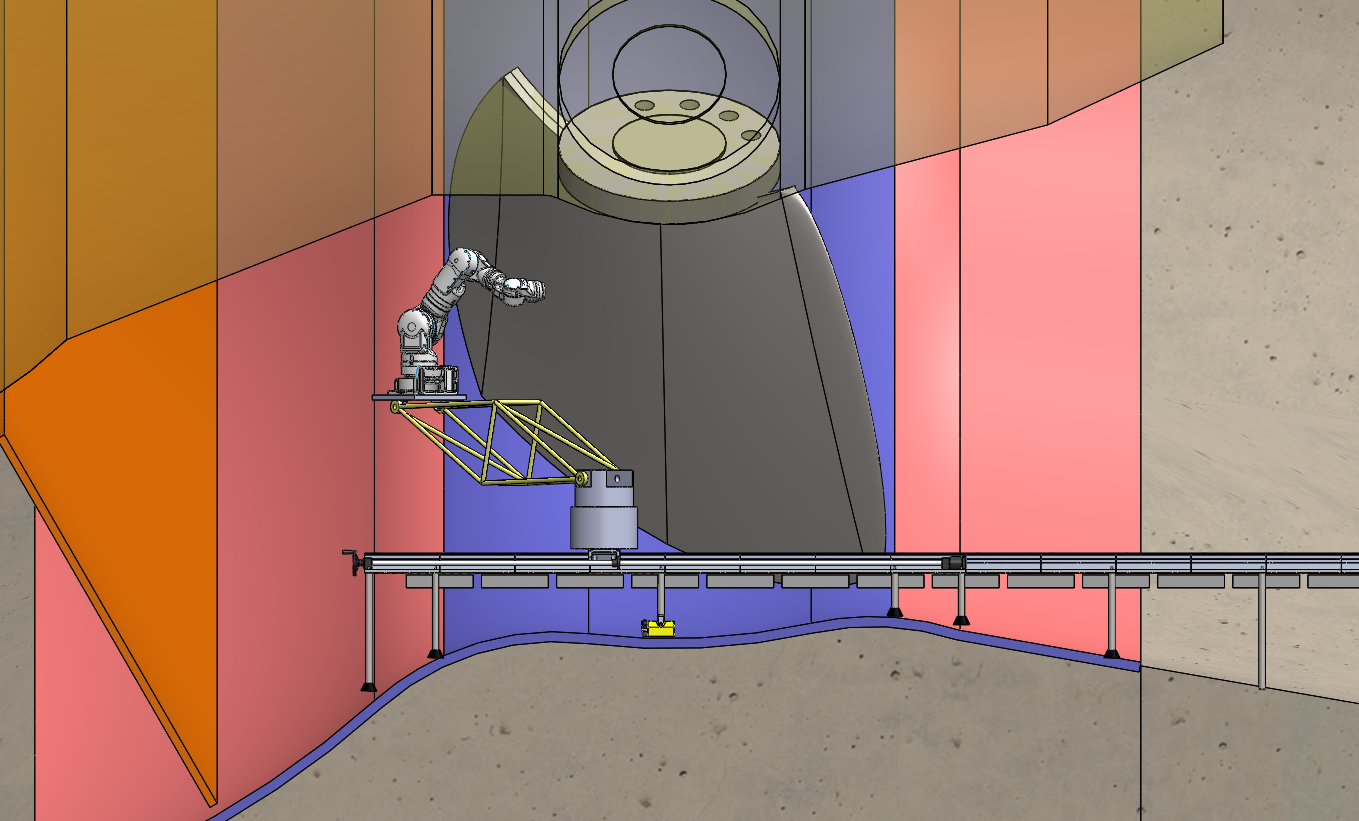
\includegraphics[width=0.8\columnwidth]{figs/bases/base_prr}
   \caption{Base Primático-Rotacional-Rotacional}
   \label{fig::base_prr}
\end{figure}

  A vantagem deste conceito é conferir um alcance grande ao manipulador através
  da base, permitindo que este possa ser de menor alcance próprio, mas ao mesmo
  tempo mais leve.
  Porém, devido à configuração de juntas e pelos resultados encontrados no
  estudo cinemático, a manobrabilidade desta base seria reduzida naquele espaço,
  havendo posicionamentos difíceis de serem alcançados, ou até impossíveis
  dependendo do manipulador escolhido.
  
$\bullet$~\textbf{Base Prismática (P):}

  Este conceito consiste de um trilho (junta prismática) para o transporte do
  manipulador desde a escotilha até o ponto de interesse para revestimento na
  face anterior ou posterior da pá. Quando posicionado, remove-se a seção
  do trilho na direção que obstrui a rotação do rotor. Neste conceito,
  adiciona-se um grau de liberdade ao sistema utilizando a própria rotação do
  rotor, posicionando a pá em relação ao robô. A base mecânica então forneceria
  apenas movimento no trilho na direção do eixo da turbina, deixando fixas as
  outras direções. O procedimento para o revestimento seria o posicionamento do
  rotor, deixando a região a ser processada ao alcance do manipulador; o
  posicionamento do robô no trilho, em relação a pá; a ancoragem do robô
  no ambiente; e o revestimento da região possível para aquela posição.
  Repete-se então este procedimento até ter toda a face processada e
  posiciona-se a próxima pá para revestimento, sem necessidade de mover ou
  desmontar a base do robô até todas as faces daquele lado estarem completas.  A
  figura~\ref{fig::base_p} ilustra este conceito.
  
  \begin{figure}[h!]
   \centering
   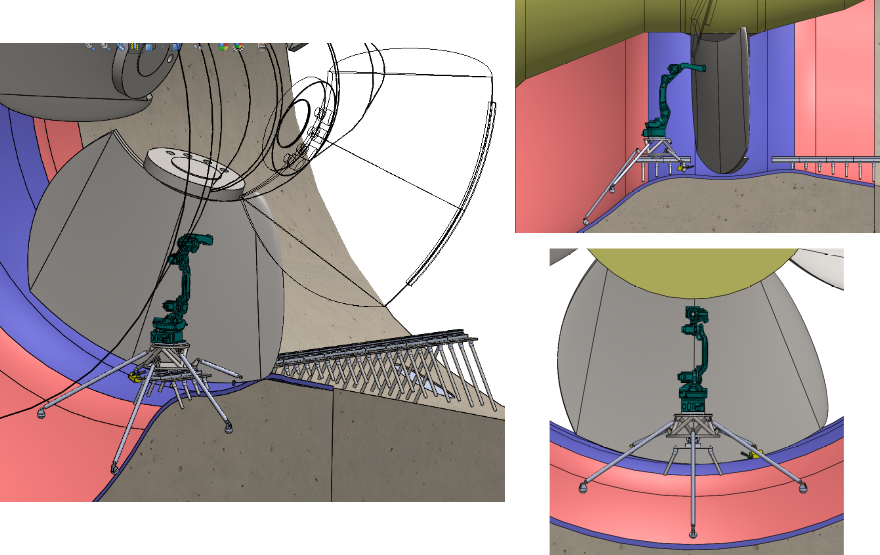
\includegraphics[width=0.8\columnwidth]{figs/bases/base_p}
   \caption{Base Prismática}
   \label{fig::base_p}
\end{figure}
  
  Este conceito foi estudado para o manipulador MH$12$, que de acordo com a
  análise cinemática consegue processar toda a extensão vertical. Para outros
  manipuladores, seria necessário incluir uma junta prismática, adicionando um
  grau de liberdade, na direção vertical.
  
  A análise cinemática também demonstrou que seriam necessárias muitas posições
  do rotor para completar uma face da pá. Há inclusive dificuldades operacionais e
  de segurança no procedimento de rotação do rotor que devem ser considerados. O
  rotor só pode ser girado manualmente, não fornecendo precisão no
  posicionamento da pá em relação a base. Por ser uma tarefa manual, deve-se ter
  procedimentos adequados de segurança para preservar tanto o operador quanto os
  equipamentos próximos. Estas preocupações tornam a solução pouco prática sob o
  ponto de vista operacional.

$\bullet$~\textbf{Base Prismática-Rotacional-Prismática (P-R-P):}

  Este conceito consiste de uma base composta por um trilho primário (junta
  prismática $1$), uma plataforma de base pivotada por mancal e rolamentos entre
  o trilho primário e secundário (junta rotacional) e um trilho secundário
  (junta prismática $2$). Montado o trilho primário alinhado ao eixo da turbina
  a base rotacional sobre o trilho primário, fixa-se o robo sobre a base
  rotacional. Esta base permitrá a montagem do trilho secundário apenas quando o
  robô atingir a região de interesse para revestimento. Quando posicionado o
  manipulador, monta-se então o trilho secundário alinhado ao plano paralelo a
  face da pá e ancora-se a base no ambiente. Desta forma, o robô pode-se
  movimentar ao longo de toda a extensão da pá por meio do trilho secundário e
  também se aproximar e se afastar da superfície da pá, por meio do trilho
  primário. A figura~\ref{fig::base_prp} ilustra este conceito.

\begin{figure}[h!]
   \centering
   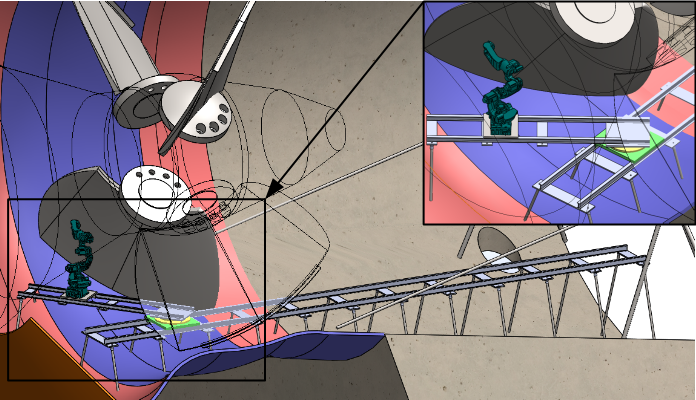
\includegraphics[width=0.9\columnwidth]{figs/bases/base_prp}
   \caption{Base Primática-Rotacional-Prismática}
   \label{fig::base_prp}
\end{figure}

  Desta forma, o rotor deve estar girado em, no mínimo $30^o$ para não haver
  contato com o trilho primário. A análise cinemática será realizada para
  encontrar a melhor configuração de juntas da base que permite ao robô se
  movimentar nos graus de liberdade da base, sem alterar o posicionamento do
  rotor e, assim, cobrir uma face inteira da pá. Para a repetição do processo
  nas outras pás do lado da sucção da turbina, é necessária a desmontagem do
  trilho secundário, o recuo do robô e desmontagem de parte do trilho primário,
  permitindo o giro do rotor para a pá seguinte.
  Para as faces do lado de adução, não é necessária a desmontagem parcial do
  trilho primário. 
 
\subsubsection{Sistemas de elevação, fixação e ancoragem}
A entrada dos componentes da base mecânica é uma tarefa trabalhosa, devido ao
acesso limitado ao interior da turbina. O diâmetro de $800~mm$ da escotilha
inferior limita o tamanho e geometria dos equipamentos, fazendo com que estes
tenham dimensões reduzidas.
Estes componentes devem ser içados até a escotilha em uma altura de $5~m$ entre
o piso no exterior do ambiente confinado e seu interior. Assim, a modularidade dos elementos que compõe a base
é uma diretriz essencial a esse projeto. A estratégia então é ter-se pequenos módulos de componentes
que poderão ser içados separadamente e acoplados entre si, até se obter a
estrutura completa. 
A facilidade de transporte, montagem e desmontagem da base mecânica causará um
grande impacto na praticidade e agilidade de implementação da solução.

A entrada de pessoal através da escotilha é feita por uma escada vertical com
guarda-corpo. Equipamentos de segurança como
cinto e talabarte devem ser usados para qualquer um que deseja entrar no
ambiente confinado da turbina através da escada e isso impossibilita o
transporte manual dos equipamentos. Por este motivo, deve ser instalada uma
estrutura com talha que permita a elevação até o interior da turbina e
movimentação para a áera de montagem adequada. As figuras~\ref{fig::talha} e
\ref{fig::talha_trilho} ilustram a estrutura de elevação com talha e carro
trole. 
  
\begin{figure}[h!]
   \centering
   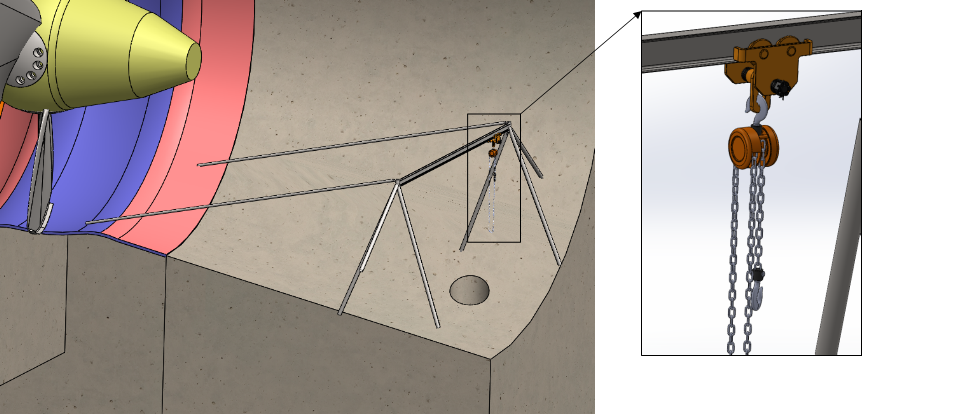
\includegraphics[width=0.8\columnwidth]{figs/bases/talha}
   \caption{Sistema de elevação dos equipamentos}
   \label{fig::talha}
\end{figure}

\begin{figure}[h!]
   \centering
   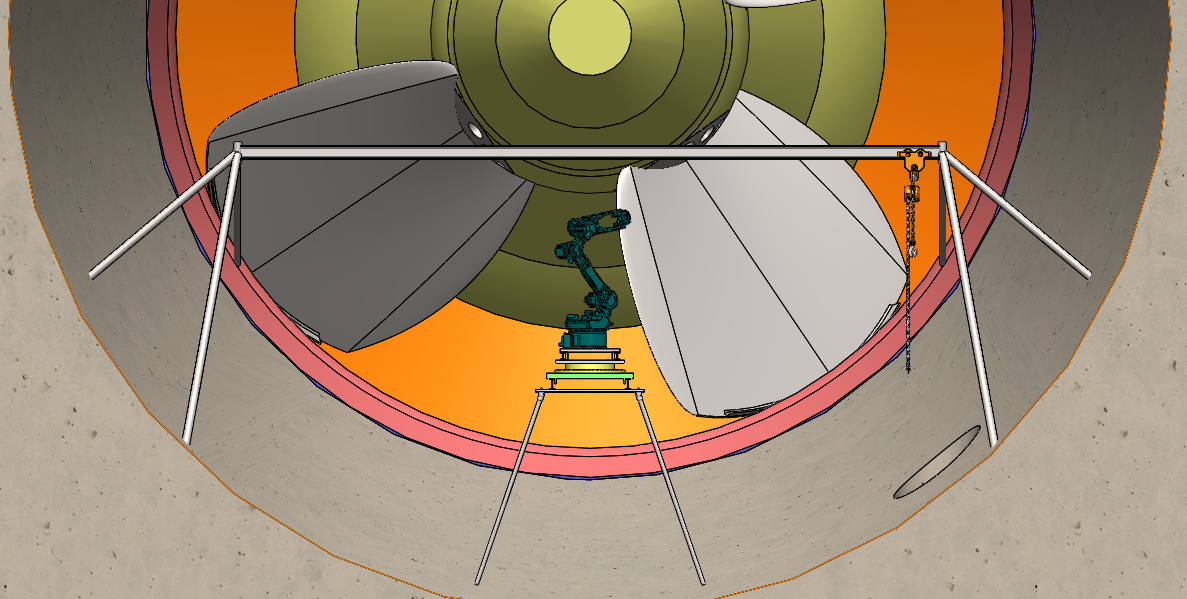
\includegraphics[width=0.8\columnwidth]{figs/bases/talha_trilho}
   \caption{Visão frontal da talha e trilho}
   \label{fig::talha_trilho}
\end{figure}

Devido aos esforços dinâmicos de operação do robô, a fixação da estutura da
base mecânica no ambiente deve ser dimensionada com cuidado. Por se
tratar de um ambiente de escoamento de fluido sob pressão, não são admitidas
modificações permanentes de infra-estrutura no interior da turbina, logo,
qualquer método de fixação utlizado deve ser removível, sem causar nenhum dano
à qualquer superfície. Em visita técnica realizada em Outrubro de $2015$ foi
testada a viabilidade de utlização de bases magnéticas para o sistema de
ancoragem e fixação. Este teste teve o objetivo de verificar a real carga limite de tração
do imã, considerando o ambiente (geometria), materiais e acabamentos
superficiais reais a que estará submetido na solução final. O resultado
detalhado do teste encontra-se no Apêndice~\ref{ape::magnetic}.

Outra opção para fixação provisória seria a soldagem da estrutura na
superfície do túnel. Esta opção segue como uma alternativa ainda para regiões
de difícil fixação da base magnética.

%%%%%%%%%%%%%% INTRO %%%%%%%%%%%%%%%

O processo de metalização utilizado atualmente considera que a posição e
orientação da pá é fixa em relação ao robô e, uma vez, que corretamente
posicionado, o processo é executado em malha aberta. Entretanto, para qualquer
uma das soluções propostas por esse documento, não é possível assumir que nem a
posição nem a orientação do manipulador, em relação a pá a ser processada, se
manterão fixas.

Para um correto planejamento de trajetória que o manipulador deve seguir durante
a tarefa de metalização, é importante o conhecimento da transformada entre o
sistema de coordenada do manipulador e da pá a ser processada. Portanto, é
necessário utilizar algum sistema que possibilite a aquisição de informações a
respeito do ambiente e da posição relativa entre o manipulador e as pás.

%%%%%%%%%%%%%%%% MKT %%%%%%%%%%%%%%%

\subsection{Estudo de sensores}

A utilização de um sensor de aquisição de dados espaciais não se limita somente
a localização, mas, dependendo do sistema a ser escolhido, pode também ser útil
na reconstrução do modelo do perfil hidráulico da pá, tanto do perfil ideal
quanto do estado atual da pá a ser processada (Tarefas descritas em
\ref{sec::introducao}).

Esta seção irá apresentar os segmentos de sensores que possam suprir essa
necessidade, assim como suas vantagens e limitações. 


\subsubsection{3D scanners}

3D scanners são equipamentos de alta precisão utilizados na indústria
geralmente em aplicações de metrologia, construção civil, monitoramento de
deformações, entre outras. O equipamento consiste em um feixe de laser que é
direcionado por meio de um espelho e a partir da mudança de fase do sinal
refletido é possível calcular a distância até o objeto atingido. O seu preço
esta na faixa de U\$70.000,00.

\paragraph{Estações de medição}

Esse tipo de sensor funciona a partir de um único feixe laser que é direcionado
por um espelho giratório acoplado a um motor de passo de alta resolução. O
sensor possui também uma base giratória, realizando assim um escaneamento de
$360^o$ do ambiente. Graças a sua construção, esse tipo de sensor possui uma
alta densidade de pontos e resolução, porém sua taxa de atualização não é muito
alta.

\begin{itemize}
  \item \textbf{Faro Focus X 330}
  	\begin{itemize}
  		\item Campo de visão (vertical/horizontal): $300^o$/$360^o$
  		\item Alcance: 330m
  		\item Velocidade máx. de escaneamento: 976.000pts/s
  		\item Precisão: $\pm$2mm
  		\item Peso: 5,2 kg
  		\item Tamanho: 240 x 200 x 100 mm
  		\item Vida da bateria: 4,5 horas
  		\item Temperatura ambiente: $5^o$ - $40^o$ C
  		\item Preço: U\$70.000,00
	\end{itemize}
  \item \textbf{Leica P16}
  	\begin{itemize}
  		\item Campo de visão (vertical/horizontal): $270^o$/$360^o$
  		\item Alcance: 40m
  		\item Velocidade máx. de escaneamento: 1.000.000pts/s
  		\item Precisão: $\pm$3mm
  		\item Peso: 12,25 kg
  		\item Tamanho: 238 x 358 x 395 mm
  		\item Vida da bateria: 5,5 horas
  		\item Temperatura ambiente: $-20^o$ - $50^o$ C
  		\item Preço: U\$80.000,00
	\end{itemize}
   \item \textbf{Nikon MV330}
  	\begin{itemize}
  		\item Campo de visão (vertical/horizontal): $45^o$/$360^o$
  		\item Alcance: 30m
  		\item Velocidade máx. de escaneamento: 2000pts/s
  		\item Precisão: $\pm$0.5mm
  		\item Peso: \textit{não informado}
  		\item Tamanho: \textit{não informado}
  		\item Vida da bateria: \textit{não informado}
  		\item Temperatura ambiente: \textit{não informado}
  		\item Preço: U\$355.000,00
	\end{itemize}


\end{itemize}


\begin{figure}[h!]
	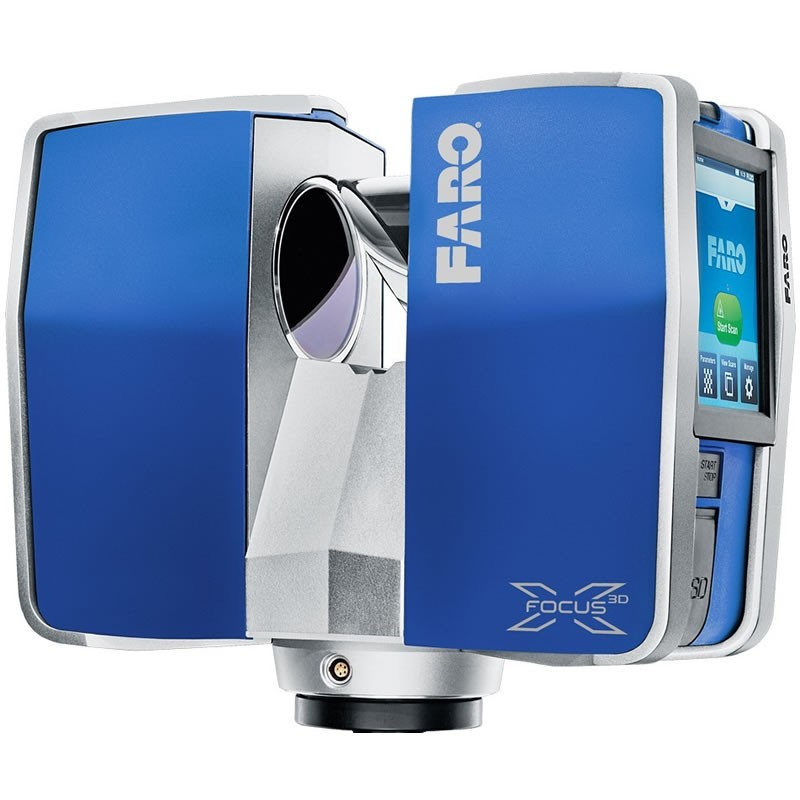
\includegraphics[width=0.6\columnwidth]{figs/3dsensors/faro}
	\caption{Sensor Faro Focus X330}
    \label{fig::faro_focus}
\end{figure}

%TODO acertar figura

\paragraph{Velodyne}

A empresa Velodyne possui, atualmente, 3 modelos de 3D Lidar. Os modelos variam
basicamente no número de pares de emissores e receptores e, consequentemente, na
resolução final. Os modelos são o VLP-16, o HDL-32E e HDL-64E, com 16,32 e 64
canais respectivamente. Esse tipo de sensor possui uma alta taxa de
atualização, entretanto não possui uma alta densidade de dados. O modelo mais
utilizado é o intermediário HDL-32E.

\begin{itemize}
\item 32 pares laser/detector  
\item Campo de Visão: +10.67$^o$ to -30.67$^o$ (vertical)
\item Rotação de $360^o$
\item Alcance - 1m - 100m 
\item 10 Hz frame rate (selecionável 5-20Hz)
\item Temperatura de Operação $-10^o$ to $+60^o$ C
\item Acurácia: $<$2 cm
\item Resolução Angular (vertical) 1.33$^o$
\item Peso: HDL-32E = 1kg; Cabos = 0.3kg
\item Tamanho: 15cm altura x 8.6cm diâmetro
\item Proteção: IP67
\item Correção de orientação (internal MEMS acelerometros and gyros)
\end{itemize}

\begin{figure}[h!]
   \centering
   \includegraphics[width=0.8\columnwidth]{figs/3dsensors/velodyne}
   \caption{Velodyne Models}
   \label{fig::velodyne_models}
\end{figure}

\paragraph{Forecast 3D Laser System}


O sensor Forecast 3D consiste em um senor 2D laser da SICK, modelo LMS 151 ou
511, acoplado a uma unidade $pan-tilt$. O seu preço esta na faixa de
U\$37.000,00.


\begin{figure}[h!]
   \centering
   \includegraphics[width=0.8\columnwidth]{figs/3dsensors/forecast}
   \caption{Forecast 3D Laser System}
   \label{fig::forecast}
\end{figure}

\subsubsection{ToF Cameras}

Conhecidas como Time-of-Flight Cameras, são dispositivos compostos por apenas
uma câmera, não necessitando de uma configuração estéreo para triangularização
de imagens. Esse tipo de dispositivo utiliza uma fonte infra-vermelho interna e de
forma análoga aos dispositivos laser, calcula a distância a partir da diferença
de fase do sinal refletido. Entretanto, essa tecnologia possibilita o cálculo
simultâneo das distâncias de cada objeto na região iluminada pela fonte IR,
mesmo que com resoluções limitadas.

\paragraph{Mesa Imaging SwissRanger SR4000}


\begin{itemize}
  \item Alcance para detecção: 0.1 - 10.0 m
  \item Alcance calibrado: 0.8 - 8.0 m
  \item Drift com a temperatura (T) - $\leq$ 1.5 mm/$^o$C (max.) - For 10$^o$C
  $\leq$ T $\leq$ 50$^o$C
  \item Tamanho: 65 x 65 x 76 mm
  \item Peso: 510 g
\end{itemize}

\begin{figure}[h!]
   \centering
   \includegraphics[width=0.8\columnwidth]{figs/3dsensors/mesa2}
   \caption{Mesa Imaging SwissRanger SR4000}
   \label{fig::mesa}
\end{figure}

\paragraph{Sentis M100 / Argos 3D - P100}

\begin{itemize}
  \item Medidas de distância e vídeo em tons de cinza
  \item Resolução: 160 x 120 pixels
  \item 40 - 160 fps
  \item Alcance: $>$3m  (extensível até 10m indoor)
  \item Campo de Visão: $90^o$
  \item Tamanho: 75 x 57 x 26 mm
  \item Peso:
\end{itemize}

\begin{figure}[h!]
   \centering
   \includegraphics[width=0.8\columnwidth]{figs/3dsensors/argos3dp100}
   \caption{Sensor Argos 3D - P100}
   \label{fig::forecast}
\end{figure}

\subsubsection{Câmeras de Luz Estruturada}

Estes sensores constituem de uma fonte emissora de infra-vermelho e um receptor.
Um padrão é projetado na cena a ser reconstruida e a partir da distorção desse
padrão é possível o cálculo de distâncias. 

%TODO exemplos dos sensores de luz estruturada
%TODO Pros e cons

%TODO ELAEL - decidir se abre uma subseção d eaplicações ou coloca um exemplo de
% aplicação em cada componente - utilizar o seu material do SOTA em 3D sensors. 

\begin{center}
\begin{tabular*}{\columnwidth}{l @{\extracolsep{\fill}} cc}
\hline
{\bf Características}           &
{\bf\begin{tabular}[x]{@{}c@{}}Luz\\Estruturada\end{tabular}} & {\bf ToF}                                               \\ \hline {\bf Complexidade de Software}  & Média                                                      & \cellcolor[HTML]{92D050}{\color[HTML]{000000} {\bf Baixa}} \\
{\bf Custo Material}            & \cellcolor[HTML]{FE0000}{\color[HTML]{FFFFFF} {\bf Alto}}  & Médio                                                      \\
{\bf Tamanho}                   & Grande                                                     & \cellcolor[HTML]{92D050}{\bf Pequeno}                      \\
{\bf Tempo de Resposta}         & \cellcolor[HTML]{FE0000}{\color[HTML]{FFFFFF} {\bf Alto}}  & \cellcolor[HTML]{92D050}{\bf Baixo}                        \\
{\bf Acurácia da Profundidade}  & \cellcolor[HTML]{92D050}{\bf Alta}                         & Média                                                      \\
{\bf Qualidade com Pouca Luz}  & \cellcolor[HTML]{92D050}{\bf Boa}                          & \cellcolor[HTML]{92D050}{\bf Boa}                          \\{\bf Qualidade com Muita Luz} & \cellcolor[HTML]{FE0000}{\color[HTML]{FFFFFF}
{\bf Fraca}} & \cellcolor[HTML]{92D050}{\bf Boa}                          \\
{\bf Consumo de Energia}        & Médio                                                      & \cellcolor[HTML]{92CDDC}{\bf Escalavel}                    \\
{\bf Alcance}                   & \cellcolor[HTML]{92CDDC}{\bf Escalavel}                    & \cellcolor[HTML]{92CDDC}{\bf Escalavel}                    \\ \hline
\end{tabular*}
\captionof{table}{Comparativo Luz Estruturada vs ToF. Fonte: \citep{larrylitof}}
%\caption{Dados principais do processo de metalização HVOF}
\label{tab::estructvstof}
\end{center}

\subsection{Conclusão}

As restrições apresentadas pelo problema de calibração, dentro do ambiente da
turbina, impõem um conjunto de requisitos mínimos que o sensor deve apresentar:

\begin{itemize}
  \item Alta resolução
  \item Portabilidade
  \item Alcance suficiente (>20m)
  \item Resistir as condições de temperatura e umidade 
\end{itemize}

Além desses requisitos, é desejável também que o sensor tenha alimentação
idependente e que sua velocidade de escaneamento não seja um fator limitante
para a eficiência do processo.

A classe de sensores que atende todas essas condições é a das Estações de
medição, com exceção do sensor Nikon MV 330 que não possui a portabilidade
necessária para a solução proposta, além de ter um preço muito maior que de seus
concorrentes.

O sensor Faro Focus X330, além de satisfazer os requisitos mínimos, é o que
possui menor preço e, por isso, foi escolhido como o o sensor a ser utilizado na
calibração do sistema e reponsável por colher os dados espacias do ambiente da
turbina e do robô. 

Entretanto, pelas especificações do sistema não foi possível garantir a perfeita
operação do sensor nas condições de alta umidade apresentada no interior da
turbina. O dipositivo opera com um sistema de lentes e lasers e, caso apresente
condensação em um desses componentes, o resultado final de sensoriamento pode
ser prejudicado. Devido a este fato, foi realizado uma bateria de testes na
Usina de Jirau, no interior de uma turbina, afim de confirmar a viabilidade
técnica desse sensor.

O teste realizado constituiu na utlização de quatro esferas reflexivas,
representadas na figura \ref{fig::esferas}, distribuidas pelo ambiente da
turbina.
Em seguida, foram realizadas 4 coletas de dados, sendo 3 delas à jusante do
rotor e uma entre as pás do rotor e o distribuidor. Com a nuvem de pontos
coletada, foi possível utilizar a assinatura única gerada pelas esferas para
alinhar todos os conjuntos de dados em uma única imagem 3D.

\begin{figure}[h!]
\centering
	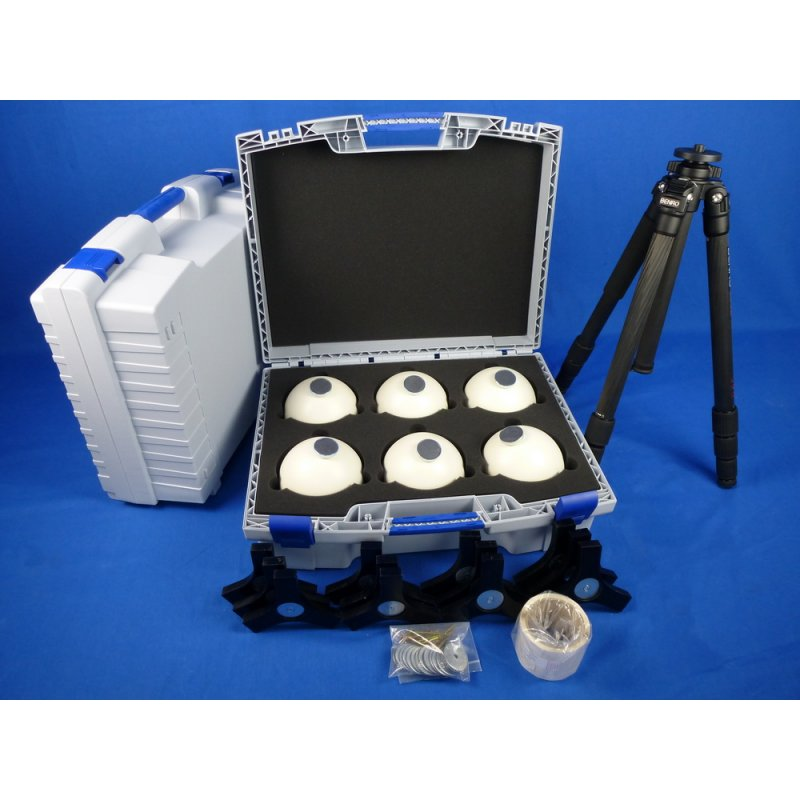
\includegraphics[width=0.9\columnwidth]{figs/3dsensors/kit}
	\caption{Conjunto de esferas reflexivas e tripé}
	\label{fig::esferas}
\end{figure}

A figura \ref{fig::turbina_faro} representa a vista frontal da imagem gerada e, por sua
vez, a figura \ref{fig::turbina_cad} representa uma reconstrução 3D gerada a
partir da nuvem de pontos coletas e utilizando o software proprietário do
fornecedor do sensor. 

\begin{figure}[h!]
\centering
	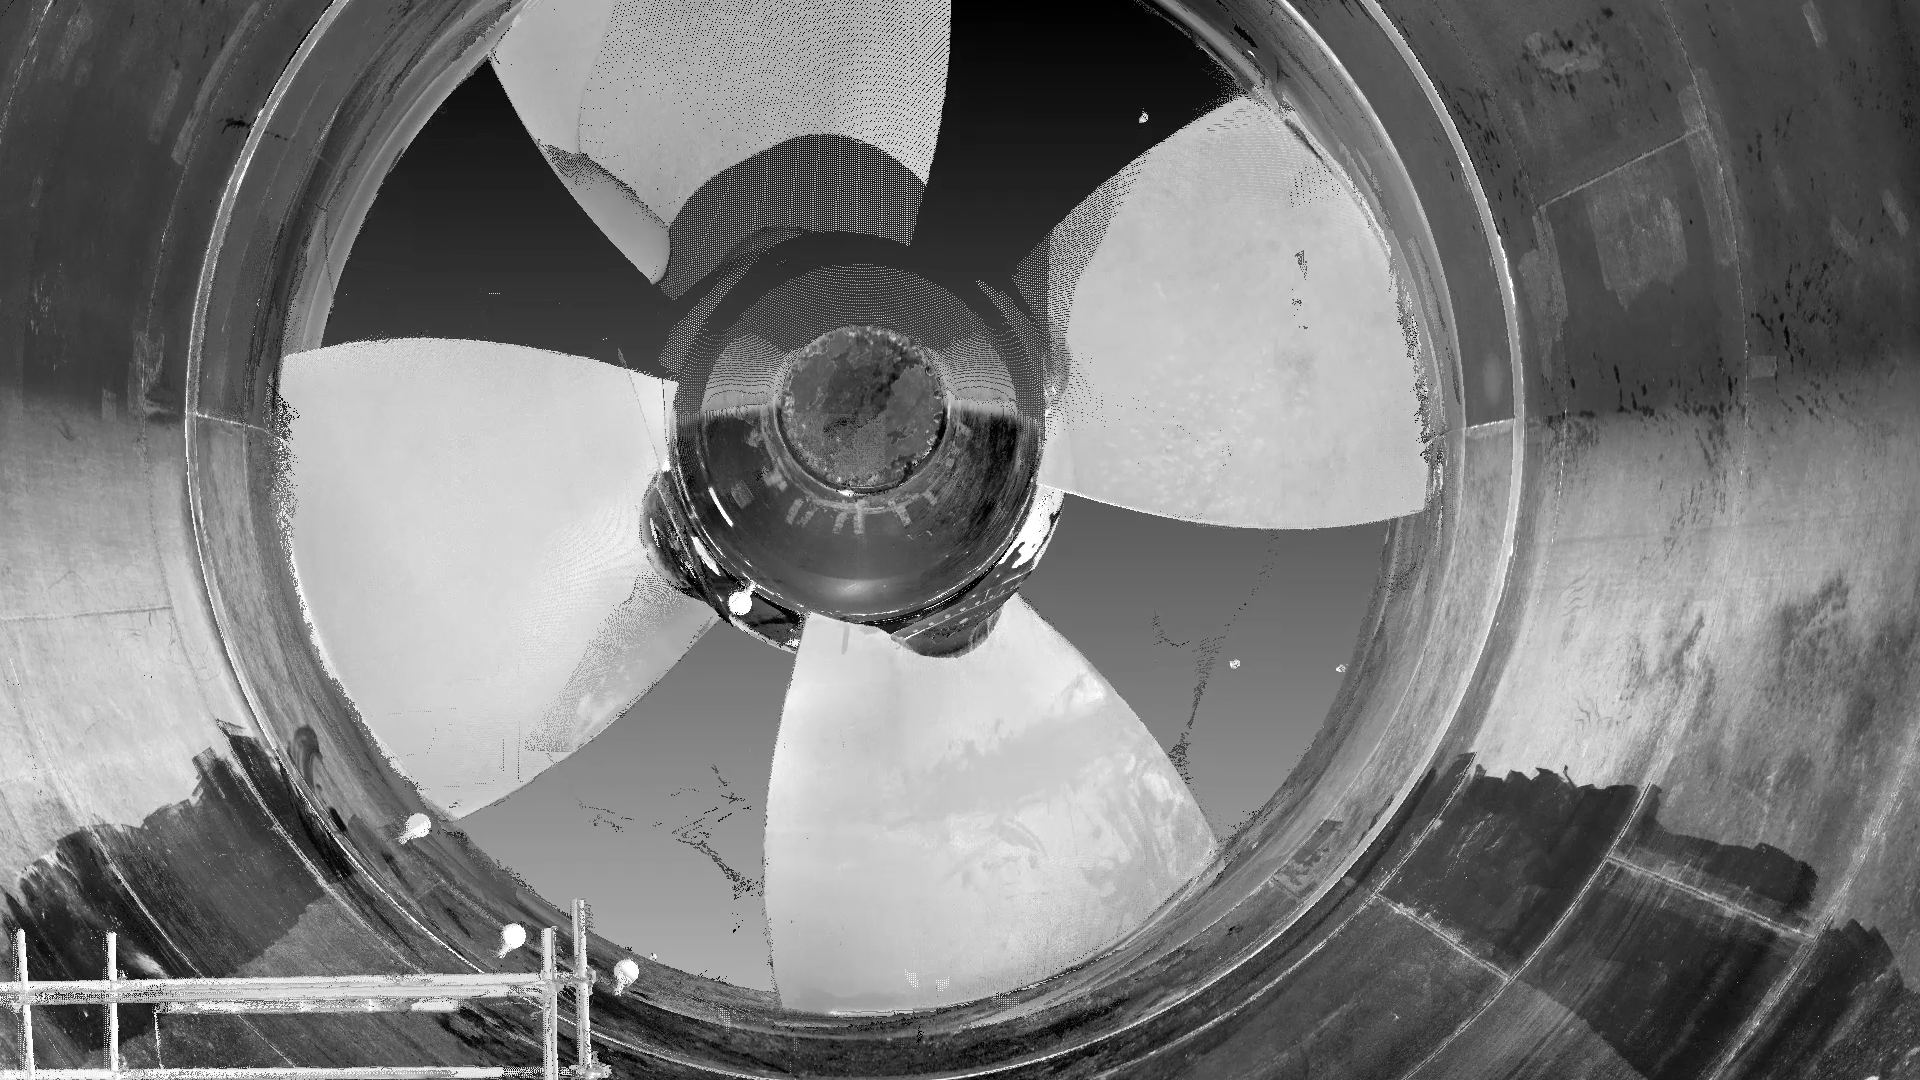
\includegraphics[width=0.9\columnwidth]{figs/3dsensors/recorte_video}
	\caption{Vista frontal da imagem gerada a partir dados adquiridos durante o
	teste.}
	\label{fig::turbina_faro}
\end{figure}

\begin{figure}[h!]
\centering
	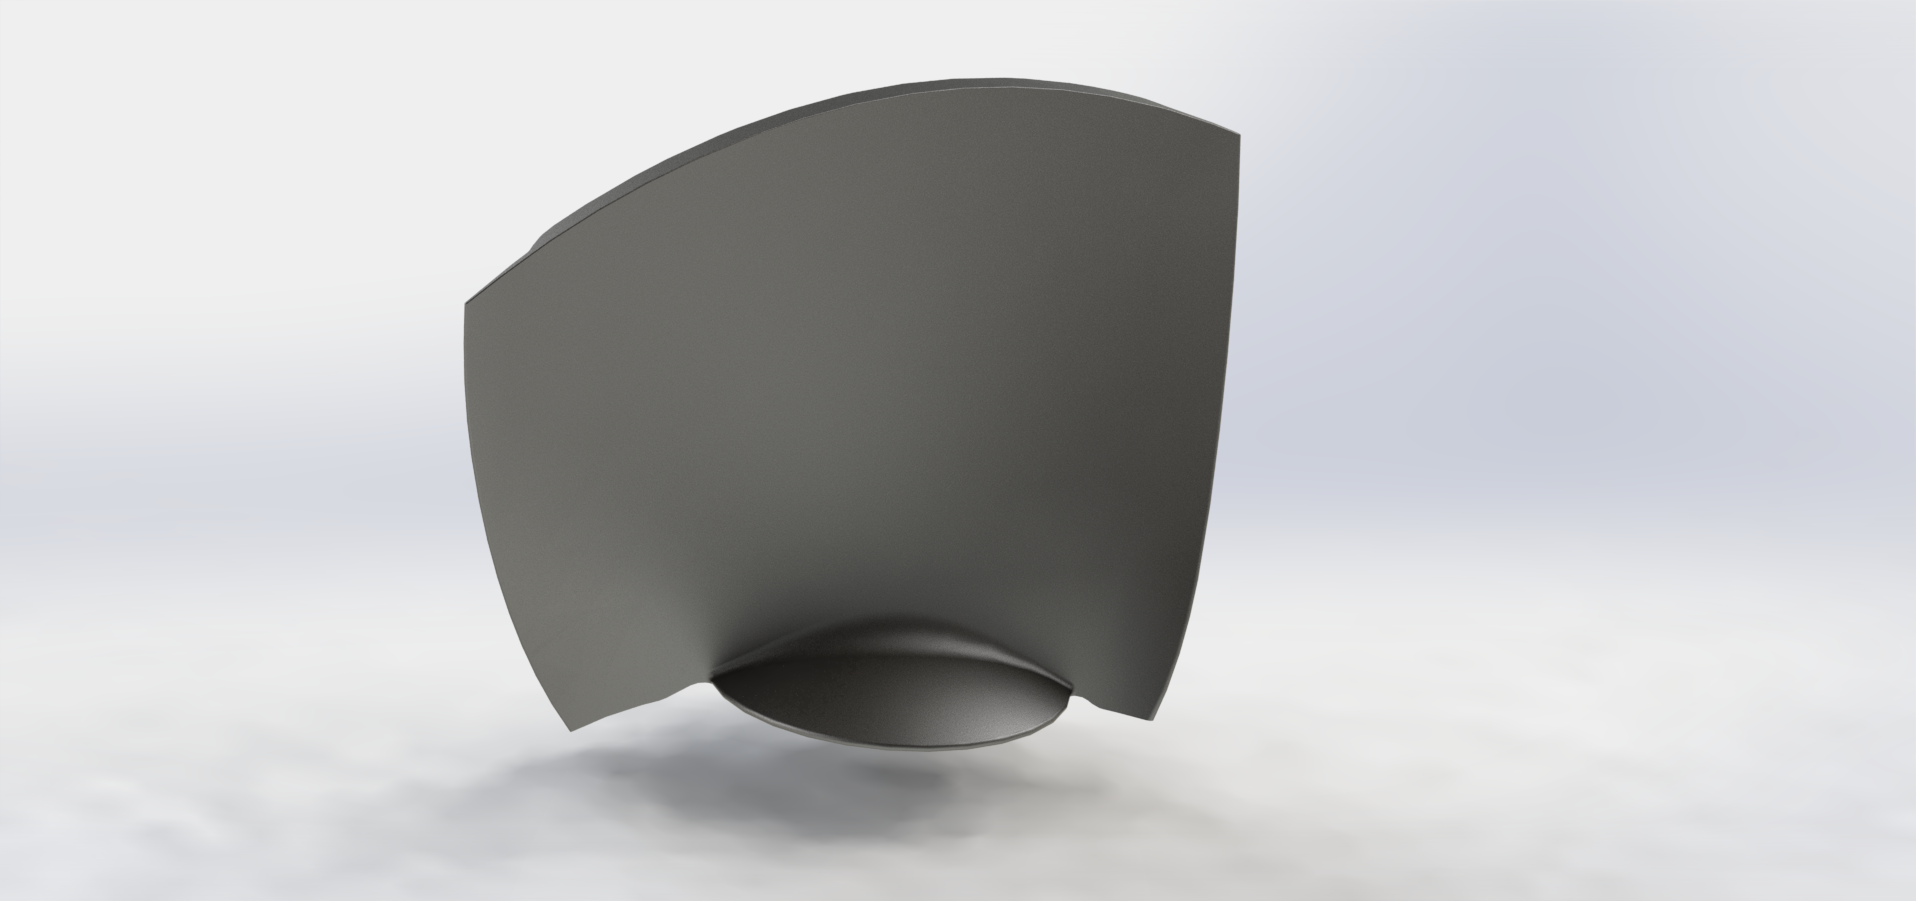
\includegraphics[width=0.9\columnwidth]{figs/3dsensors/Pa_Real_Render_04}
	\caption{Reconstrução em CAD da pá com os dados do teste.}
	\label{fig::turbina_cad}
\end{figure}

A partir dos resultados gerados durante os testes foi comprovada que o sensor é
capaz de operar nas condições extremas impostas pela turbina e com um nível de
ruído aceitável para a aplicação em questão. 


\subsubsection{Medidor de distância a Laser}

Durante o processo de metalização o 3D scanner estará desligado, pois o tempo de
varedura não o torna prático para obter informações em tempo real. Assim o
sistema estaria funcionando em \textit{loop} aberto, o que gera receios com
relação à segurança. A fim de evitar tais riscos é desejável alguma
realimentação para o sistema sobre sua posição. Essa realimentação será
realizada pelo uso de um medidor de distância a Laser, a ser posicionado próximo
à pistola de metalização, com o intuito de aferir a distância da pistola até a
pá em tempo real.

\begin{figure}[h!]
\centering
	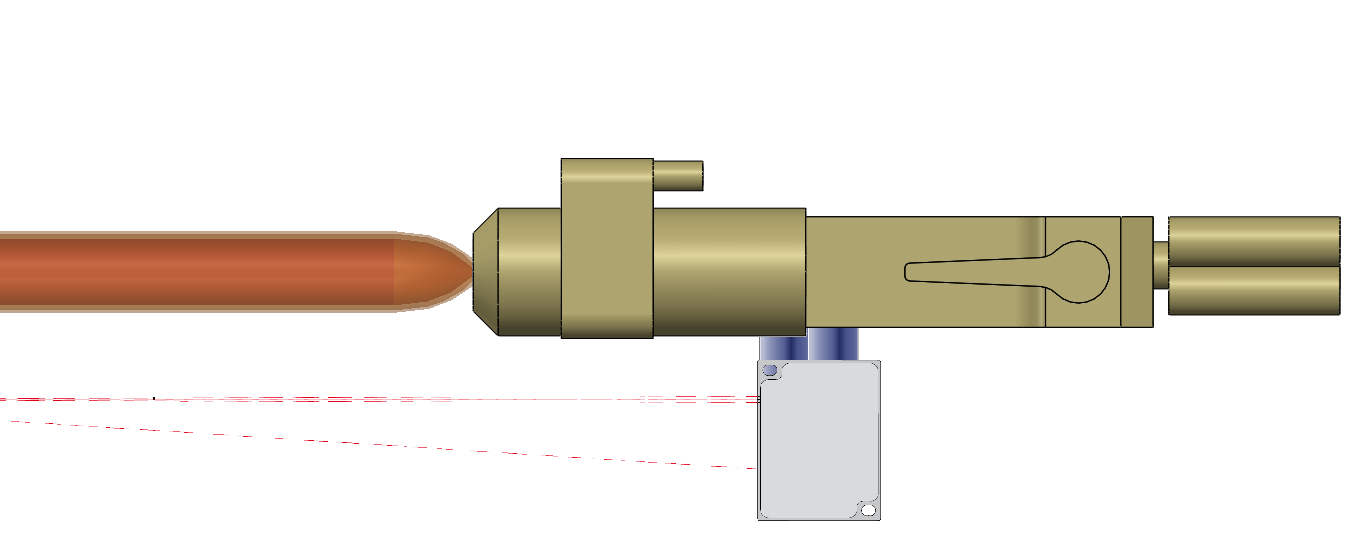
\includegraphics[width=0.9\columnwidth]{figs/3dsensors/senso_laser_pistola}
	\caption{Ilustração da posição do medidor de distância, em cinza, na pistola de
	metalização.}
	\label{fig::laser}
\end{figure}


Para a escolha de medidor compatível foram analisadas as seguintes variáveis:

\paragraph{Temperatura}
A temperatura da superfície pode influenciar na precisão do sensor devido à
radiação de corpo negro. Caso essa radiação térmica atinja níveis relevantes na
faixa de frequência do Laser utilizado ocorre degradação da qualidade de
reposta do sensor. Análises de campo identificaram que, apesar da alta
temperatura da chama de metalização, a pá da turbina não chega a emitir níveis
preocupantes de radiação na faixa do vermelho ($670 nm$), onde operam os Lasers
padrões. Para casos de exceção existem Laser que trabalham em regiões do
azul/violeta.

Por outro lado a temperatura do ambiente também influencia o sensor, que não
costuma ter alta resistência à temperatura, ficando algo em torno do $50^oC$.
Para evitar que o calor da chama seja recebido diretamente pelo sensor,
aumentando a temperatura ambiente na região, ele deve ser posicionado na pistola
com uma distância de segurança da chama (figura \ref{fig::laser}).

\paragraph{Distância de operação}
A metalização ocorre com a pistola entre 23cm e 24cm de distância da pá. Somado
a isso temos a distância do sensor à chama para então sabermos a distância da
pá ao sensor. Considerando que a pistola possui em torno de 30cm de comprimento,
a faixa de operação de distâncias do sensor deverá incluir 40-50cm. Para termos
essa região no centro da faixa de operação, ela deverá iniciar em 20-25cm e
trabalhar até 80-100cm.

\paragraph{Poeira e Umidade}
A alta umidade ambiente dentro do aro câmara, e em todo circuito hidráulico,
impõe mais um requisto sobre o equipamento. Além disso, o pó residual da
aplicação da metalização pode ser danoso ao sensor. Um isolamento apropriado
para o sensor pode ser encontrado segundo a padronização IP69K.

\paragraph{Precisão}
Como a tolerância está na ordem de milímetros ( a distância do sensor à pá deve
se manter em uma faixa de $\pm 5mm $ entre 23cm e 24cm ), logo é desejável que o
sensor possua precisão de $1mm$ ou menor.

\paragraph{Peso}
Considerando a carga máxima no punho do robô de 10kg, e a massa da pistola de
8,5kg e aplicando as restrições dinâmicas ( para manter a velocidade
desejada em todos os pontos ) conclui-se que o medido deve ter uma massa
inferior a 1kg.

%%%%%%%%%%%%%%%  TECNICAS %%%%%%%%%%%%%%%%%%%%%%

\subsection{Estudo de técnicas de reconhecimento} 

As informações de distância recebidas pelos sensores descritos na seção
anterior podem ser armazenados como uma estrutura de dados chamada nuvem de
pontos, isto é, uma representação tridimensional do espaço cartesiano, na qual cada distância medida pelos
sensores a partir de sua origem representa uma coordenada x y z.
Entretanto, essa representação não é capaz de diferenciar, ou classificar, os
limites de cada objeto presente na cena, ou seja, não é possível determinar
\textit{a priori} qual conjunto de pontos pertence a cada elemento que se deseja
identificar para realizar a calibração.

A identificação de cada conjunto, ou \textit{cluster}, de pontos é importante
para que a posição e orientação de cada objeto de interesse seja determinada e,
assim a transformação do sistema de coordenadas entre cada objeto seja
calculada. Esse processo necessita, então, do estudo e implementação de
algoritmos para a análise da nuvem de pontos, identificação dos elementos
necessários, extração de suas respectivas posições e, finalmente, cálculo da
transformação entre as posições. 

Dependendo das características de cada objeto a ser identificado e da
possibilidade de implementação de uma estrutura de apoio para facilitar a sua
identificação, podem ser utilizados diferentes métodos e estratégias de
identificação e localização, que serão exploradas a seguir.

\subsubsection{Reconhecimento do Robô}

O Robô é uma estrutura que a idenficação pode ser facilitada pelo uso de
padrões de fácil reconhecimento (como esferas e padrões de xadrez, figuras
\ref{fig::sphere_rec} e \ref{fig::checkerboard_rec} ), pois alterações na base
do robô não ocasionam problemas para o funcionamento do sistema.


\begin{figure}[h!]
   \centering
   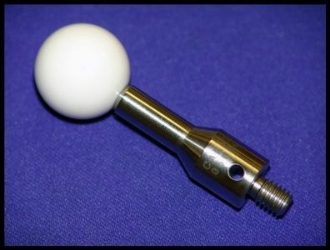
\includegraphics[width=0.95\columnwidth]{figs/localizacao/sphere_rec}
   \caption{Exemplo de esfera utilizada para reconhecimento. Fonte:
   http://shop.talwin.net/}
   \label{fig::sphere_rec}
\end{figure}



\begin{figure}[h!]
   \centering
   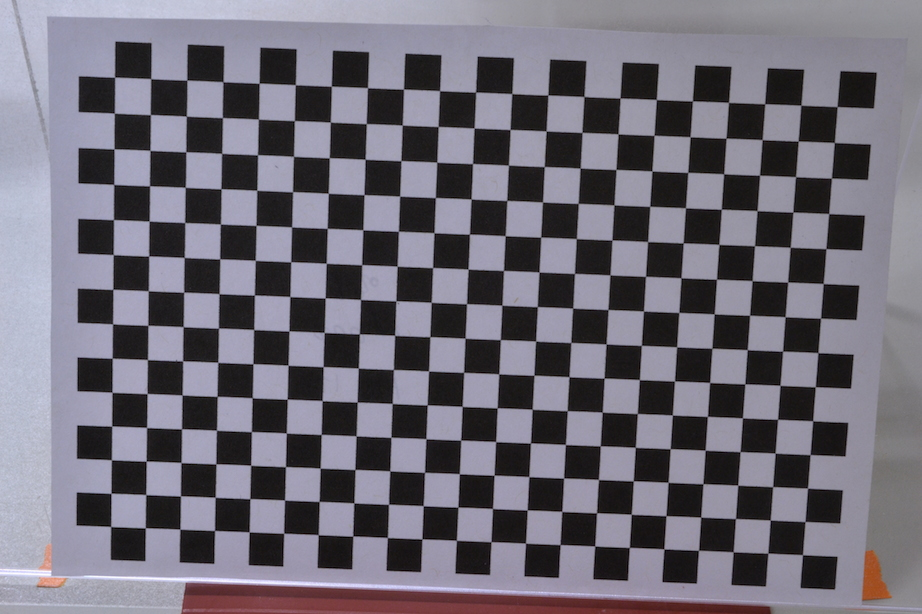
\includegraphics[width=0.95\columnwidth]{figs/localizacao/checkerboard_rec}
   \caption{Exemplo de padrão de xadrez utilizado para renhecimento.\\ Fonte:
   http://stereomorph.blogspot.com.br/}
   \label{fig::checkerboard_rec}
\end{figure}


Devido a baixa iluminação ambiente dentro do circui\-to da tubina, a opção
mais simples é o uso de nu\-vem de pontos sem identificação de cor. Ou seja, o
reconhecimento se dará apenas pelo formato. Isso restringe o uso de padrões de
xadrez e o foco se voltará, então, para o uso de formatos geométricos. Em
especial o mais simples objeto de três dimensões: a esfera.

O reconhecimento de formas geométricas simples em três dimensões é um assunto
já razoavelmente explorado na literatura. Dentre eles pode-se destacar 2
métodos: RANSAC e Hough Transform.

\paragraph{RANSAC}
O método RANSAC (acrônimo para ``RANdom SAmple Consensus", \textit{consenso por
amostragem aleatória} em tradução livre) é um método iterativo que tem como
premissa a presença de \textit{outliers} (elementos fora do corpo principal) na
amostra e objetiva a identificação dos parâmetros matemáticos que descrevem o
objeto geométrico em questão \cite{ransac}. É o método
disponível na amplamente utilizada biblioteca de processamento de nuvem de pontos ``PCL''. 

Esse método consiste na seleção aleatória de pontos para serem considerados como
partes integrantes do corpo principal (no caso, uma esfera), a partir desses os
parâmetros da esfera são calculados (comumente, os valores x, y e z do centro
da esfera e seu raio). Então os demais pontos são julgados como fazendo parte ou
não da esfera de acordo com esses parâmetros. O modelo é avaliado como bem estimado se uma quantidade razoável de pontos são considerados
como pertencentes à esfera. Se for visto como bem estimado, os parâmetros são
então reestimado levando em conta de todos os pontos que foram considerados como
pertencentes à esfera. O erro do modelo é inferido a partir dos pontos que foram
considerados como fazendo parte da esfera e uma esfera reconstruída pelos
parâmetros calculados. O processo então é repetido um número artrário de vezes,
e se mantém armazenado o modelo que obteve menor erro.

Um dos principais pontos negativos do RANSAC é que ele tem como premissa a
presença de apenas um corpo principal, ou seja, apenas uma esfera. Isso implica
em um tratamento especial quando temos mais de uma esfera no ambiente.

\begin{figure}[h!]
   \centering
   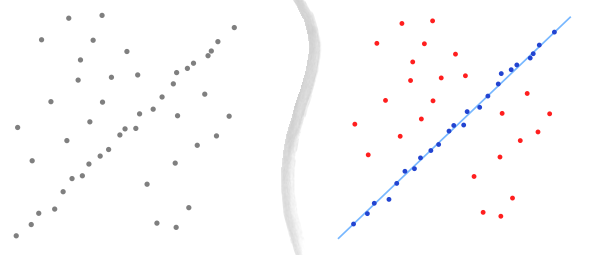
\includegraphics[width=0.95\columnwidth]{figs/localizacao/ransac}
   \caption{Exemplo de reconhecimento de uma linha em 2 dimensões usando
   RANSAC. (Fonte: \cite{ransac})}
   \label{fig::ransac}
\end{figure}
 
 \paragraph{Transformada de Hough 3D}
Anos de pesquisa em reconhecimento de objetos geométricos de duas dimensões
levaram ao desenvolvimento e aprimoramento de técnicas basedas em ``Transformada
de Hough''. Essas técnicas tem sido recentemente adaptadas para o universo de
três dimensões (ver \cite{hough2014}) e adequadamente chamadas de Transformada
de Hough 3D.

O método consiste em tranformar cada ponto do espaço 3D em uma variedade
mergulhada no espaço quadridimensional dos parâmetros da esfera ( x, y e z do
centro mais r do raio). A variedade se identifica com todas as possiveis esferas
que contém aquele ponto. O espaço de parâmetros é então restrito dentro de
certos limites e quantizado por razões de implementação (os recursos
computacionais são finitos). É definido então um acumulador, basicamente uma
função que conta quantas variedade interceptam determinada região discretizada
do espaço de parâmetros. Um algorítmo de reconhecimento de picos é aplicado
sobre o espaço de parâmetros (com as varidade já mergulhadas nele) para detectar
qual o conjunto de parâmetros que está melhor descrevendo um maior número de
pontos. O algorítmo pode ser utilizado para reconhecer mais de um pico e, assim,
identificar a presença de mais de uma esfera na nuvem de pontos (exemplo na
figura \ref{fig::hough}).

A dificuldade no uso do método é seu custo computacional, mas existem soluções
que exploram amostragens estatísticas para reduzir o custo computacional.

\begin{figure}[h!]
   \centering
   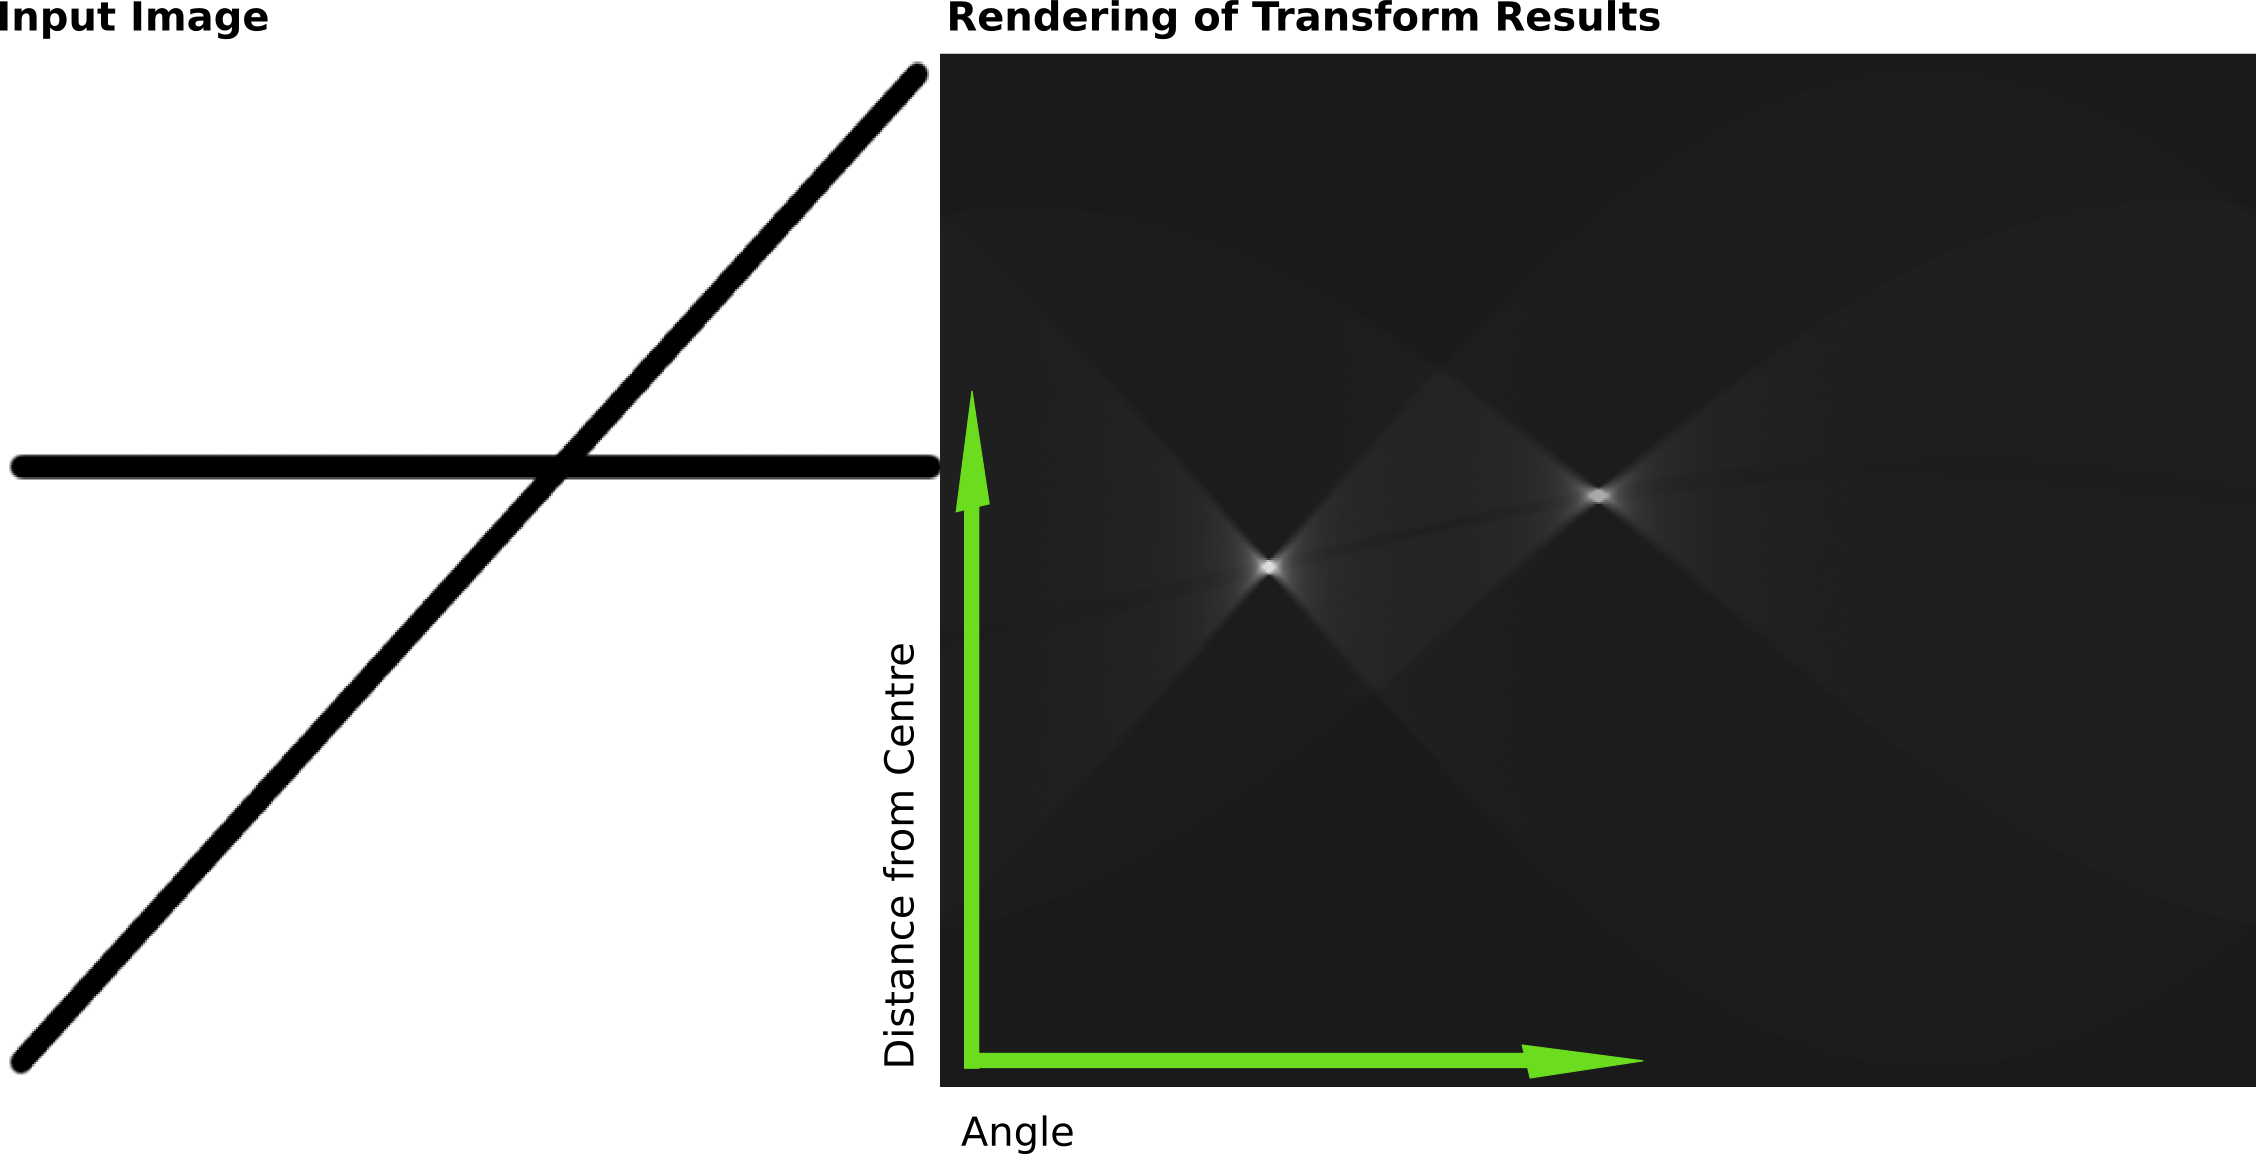
\includegraphics[width=0.95\columnwidth]{figs/localizacao/hough}
   \caption{Exemplo de reconhecimento de duas linhas em 2 dimensões usando
   Transformada de Hough. Na esquerda estão pontos que compõem as duas retas, na
   direita uma sobreposição das variedades referentes a cada ponto das retas
   (mergulhadas em um espaço paramétrico bidimensional). Os pontos mais
   brilhantes refletem os picos referentes aos parâmetros que melhor descrevem as duas retas. (Fonte: 
   \url{https://en.wikipedia.org/wiki/Hough_transform})}
   \label{fig::hough}
\end{figure}

Tendo conhecimento da posição de quatro esferas, pelo uso de um dos métodos
descritos acima, é possivel unicamente identificar a posição de um corpo preso a
elas. Em outras palavras, consegue-se a transformada entre origem do sistema de
coordenadas (tipicamente no sensor) e o robô. Para descobrir a trasnformada
entre o robô e a pá (posição relativa entre eles) falta identificar a
transformada entre a origem e a pá, esse caso será explorado na próxima seção a
seguir.

\subsubsection{Reconhecimento da Pá} 

Para a identificação e localização das pás das turbinas não é possível a
utilização de nenhum artifício de apoio que facilite o processamento da nuvem de
pontos, pois a instalação de qualquer um desses aparatos não pode ter precisão
garantida nas operações de campo. Uma instalação de um elemento de apoio em
pontos precisos da pá necessitaria também de calibração para cada utilização, retirando assim
o propósito do método. 

Portanto, para a localização das pás da turbina é
necessário explorar as características espaciais intrínsecas à superfície do
próprio objeto e identificá-las na nuvem de pontos do ambiente. O objetivo
principal nessa etapa do processo é, então, identificar um conjunto mínimo de
características do objeto que o represente unicamente com um baixo grau
de ambiguidade e sem exigir muito esforço computacional. 

A escolha do tipo de característica a se usar é uma decisão fundamental para a
eficiência do processo e tem sido alvo de estudos na literatura para a análise
e reconhecimento de imagens 2D, como imagens RGB de câmeras e mais recentemente
também para imagens 3D. 

Uma boa representação de \textit{point feature} deve ser capaz de capturar as
mesmas características locais da superfície na presença de:

\begin{itemize}
  \item \textbf{Transformadas} -  rotações e translações 3D nos dados não devem
  influenciar a estimação dos descriptors;
  \item \textbf{Variações na densidade de amostragem} - em princípio, uma de
  superfície amostrada mais ou menos densamente deve ter a mesma assinatura característica do vetor
  \item \textbf{Ruído}
\end{itemize}

O reconhecimento de objetos em aplicações robóticas também vem recebido
grande atenção, principamente com o crescimento da robótica móvel e em ambientes
não estruturados, onde é necessário identificar e localizar os objetos a serem
manipulados em cada tarefa. O problema é enfrentado basicamente utilizando-se
duas abordagens: analisar os dados 3D ou realizar algum tipo de processamento e
projeção para se trabalhar com imagens 2D e utilizar as técnicas mais maduras
desse tipo de imagem.

Nesta última categoria, a técnica
mais usada consiste em converter as informações tridimensionais em \textit{Range
Images}, na qual é realizada uma projeção a partir de um ponto de vista (geralmente o do sensor) e utiliza escala
de cores ou cinza para representar a distância, ou seja, quanto mais escuro o
objeto na imagem, mais longe ele se encontra. É importante reassaltar que esse
tipo de método introduz perdas de informação ao se realizar projeções e é
sensível à escolha do ponto de vista escolhido. 
%Em \cite{Bayramoglu2010} são
%utilizados descritores SIFT, ou \textit{Scale-Invariant Feature Transform},  
%como características a serem identificadas na imagem. \textit{Local Feature
%Histograms} são utilizados em \cite{Hetzel2001} e por sua vez \cite{Chen2007}
%optou por utilizar \textit{Local surface patches}. 
A escolha do descritor a ser
utilizado depende da aplicação e deve ser estudada a melhor opção para a nossa
solução, assim que tivermos dados aquisitados pelo sensor. Aplicações
semelhantes envolvendo identificação de objetos no ambiente tridimensional, mas
sem localizá-los, e utilizando diferentes descritores podem ser encotradas em
\cite{Bayramoglu2010,Hetzel2001,Chen2007}. Uma comparação dos descritores
utilizados para reconhecimento de objetos 2D e 3D pode ser encontrado em \cite{Zaharia2004, Weber2014}.

Após o reconhecimento do objeto, é necessário identificar a sua posição.
Em \cite{Steder2009}, o alinhamento é realizado utilizando-se a própria
\textit{Range Image} e a informação de profundidade presente na mesma. Por outro
lado, em \cite{Nuchter2005} a região onde o objeto identificado está presente é
selecionada e, por meio de \textit{raycasting} o conjunto de pontos da nuvem
pertecentes à região identificada na \textit{Range Image} é reprojetado. Após
essa segmentação, é utilizado um algoritmo de alinhamento como o ICP.

O primeiro passo para tornar possível a localização da pá é a aquisição de seus
dados espacias e a criação de uma nuvem de pontos que a represente. A
figura \ref{fig::pa_pcd} ilustra uma nuvem de pontos representando uma pá de uma das
turbinas da usina de Jirau, esse modelo foi construído utilizando-se os dados
aquisitados durante a viagem de campo e teste de sensibilidade do sensor Faro
Focus X330, como citado anteriormente. É importante ressaltar que o
modelo deve representar, se possível, todas as características pertinentes do objeto de interesse. Nesse
sentido, se faz necessário a criação de um modelo para cada tipo de pá que
deverá ser processada, ou seja pás com diferentes perfis hidráulicos possuem
modelos diferentes.


\begin{figure}[h!]
   \centering
   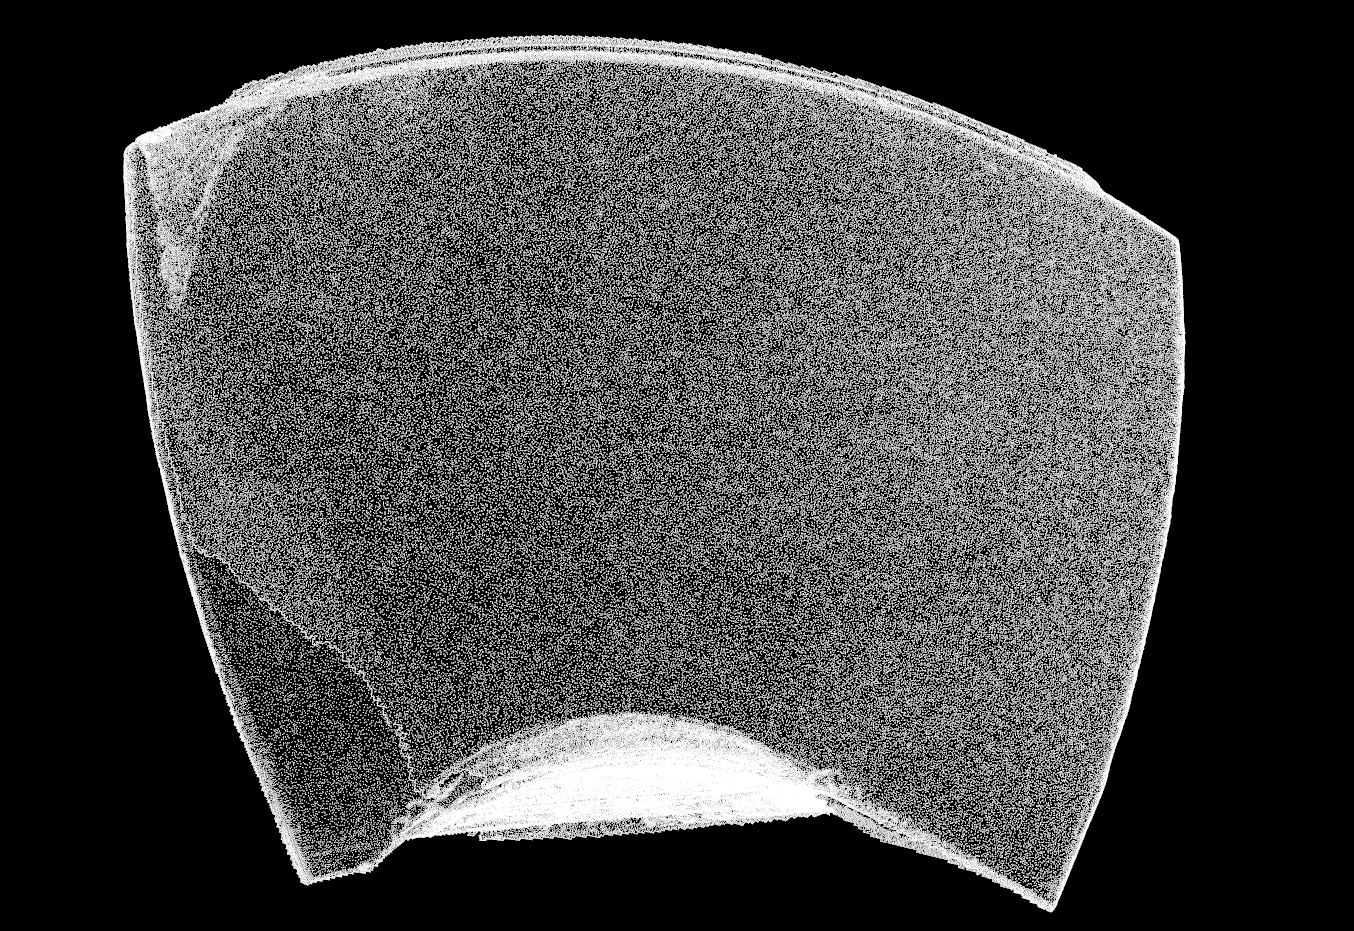
\includegraphics[width=0.95\columnwidth]{figs/localizacao/pa_pcd}
   \caption{Modelo da pá em nuvem de pontos}
   \label{fig::pa_pcd}
\end{figure}

A partir do modelo, é necessário a extração de seus pontos chaves e descritores.
A figura \ref{fig::pa_key} ilustra descritores do tipo SHOT, identificados no modelo de referência da pá. Para a nossa aplicação, não é
necessário, a princípio, o reconhecimento do objeto em questão, apenas a sua
localização e orientação no espaço tridimensional. A possibilidade de inserir no
sistema a informação de qual modelo de pá deve ser procurado, simplifica o
algoritmo e o torna menos suscetível a erros, uma vez que não é necessário
avaliar qual o modelo mais próximo das medições atuais e ainda é possível 
utilizar essa informação para fornecer uma avalição da similaridade do modelo
com os dados reais aquisitados.

\begin{figure}[h!]
   \centering
   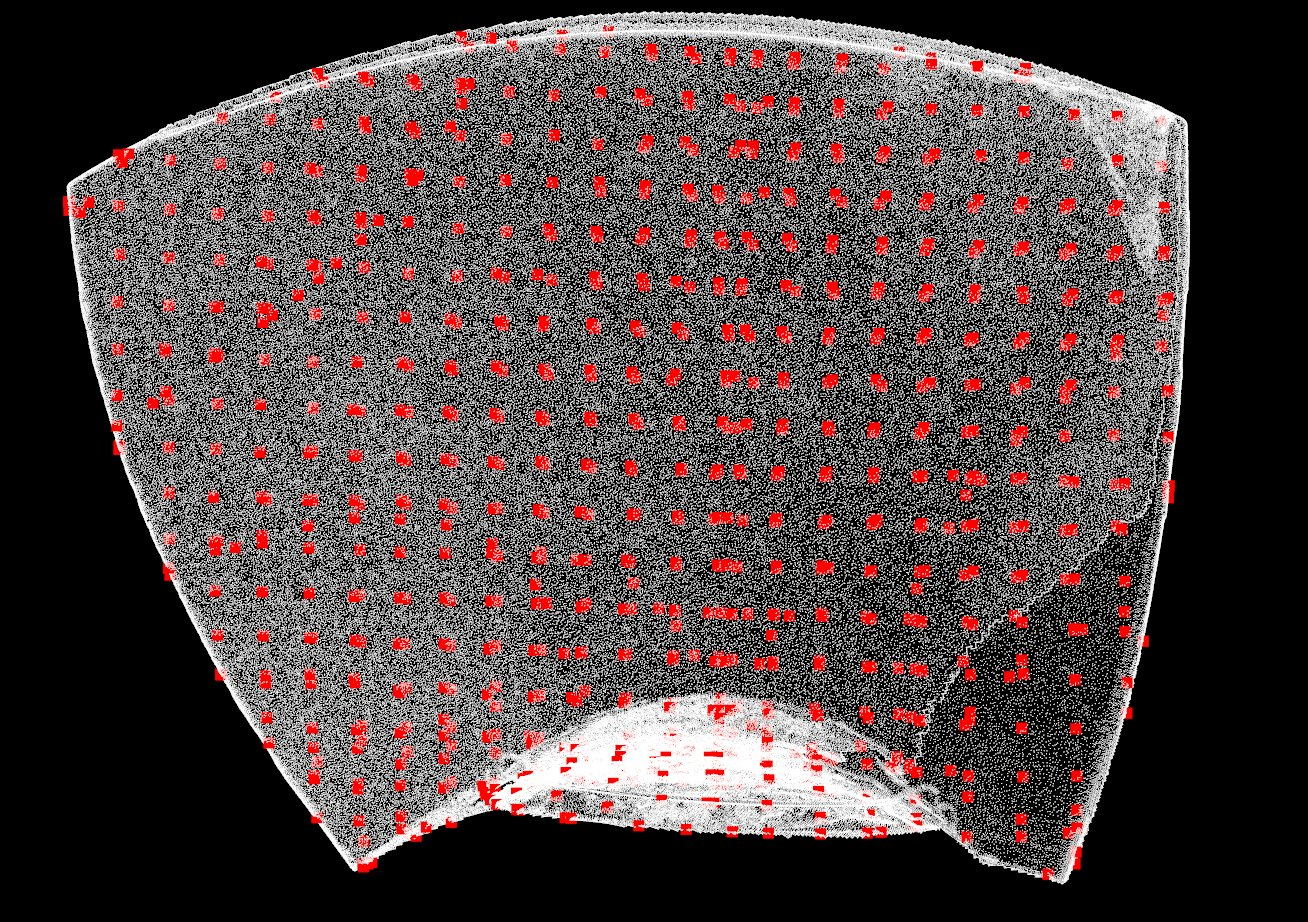
\includegraphics[width=0.95\columnwidth]{figs/localizacao/pa_key}
   \caption{Pontos de interesses com descritores associados no modelo da pá}
   \label{fig::pa_key}
\end{figure}

Uma vez que os pontos de interesse do modelo e seus descritores são extraídos, é
possível armazená-los para evitar o seu processamento  durante cada nova
calibração. Utilizando-se a estratérgia de
\textit{Correspondence Grouping} e o algoritmo \textit{Hough Voting}
\cite{Tombari2010a}, a nuvem de pontos aquisitada em campo terá também seus
pontos de interesse extraídos e um descritor associado para cada ponto. A
seguir, os descritores de ambas as nuvens, cena e modelo, são comparados afim de
se encontrar correpondentes em cada conjunto. Se um número suficiente de
correspondências é encontrado, o objeto é então detectado e localizado na
imagem. É importante ressaltar que essa técnica pode gerar falsos positivos. A
figura \ref{fig::correspondence} ilustra a implementação do algoritmo com 
dados sintéticos de uma cena, utilizando-se porém o modelo real da pá. O modelo
da pá está representado em amarelo, a pá identificada na cena em vermelho e as correspondências
conectadas pelas setas verdes.
Como próximos passos é necessário a utilização de dados reais para validação do
algoritmo e também a utilização de diferentes descritores, uma vez que apenas os
descritores do tipo SHOT foram testados.

\begin{figure}[h!]
   \centering
   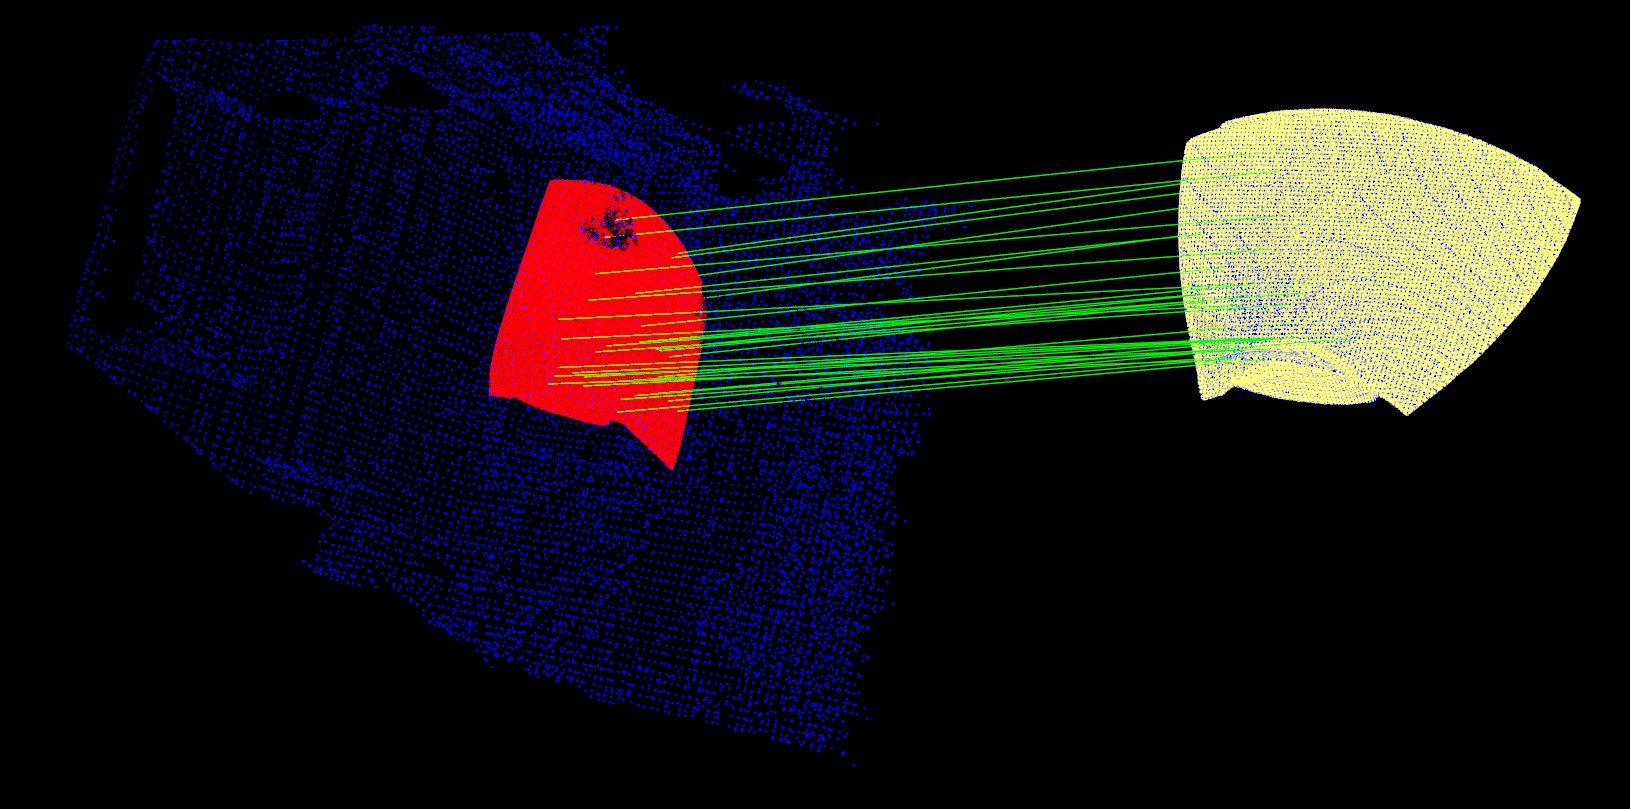
\includegraphics[width=0.99\columnwidth]{figs/localizacao/correspondence}
   \caption{Identificação e localização de uma pá utilizando
   \textit{Correspondence Grouping}}
   \label{fig::correspondence}
\end{figure}




\section{Robot Arm and Blade Covering}\label{sec:sota}
 
\input{robot_intro} 
\subsection{Pesquisa de mercado}
% Author: Renan
A pesquisa de mercado está detalhadamente explicada na
tabela~\ref{ape::bighatch}, no apêndice. Os seguintes robôs satisfazem os
requerimentos e restrições principais, de acordo com as tabelas~\ref{tab::bighatch} e ~\ref{tab::hvof}, e os requisitos abordados
em \ref{sec::desc_contex}: Viper s1300 (Adept), ARC Mate 100iC/12 (Fanuc),
M-10iA/12S (Fanuc), LBR iiwa 14 R820 (Kuka), KR 10 R1100 sixx WP (Kuka), MH6F-10
(Motoman), SIA10F (Motoman), MH12 (Motoman), SIA20D (Motoman). Destes, os
manipuladores LBR iiwa 14 R820 (Kuka) e Viper s1300 (Adept) deverão passar por adaptações para
operar em temperaturas até $40^o$C e umidade relativa no ar de $91\%$; e os
manipuladores KR 10 R1100 sixx WP (Kuka), MH6F-10
(Motoman) e SIA10F (Motoman) têm carga máxima de 10 Kg, que é o limite para o
processo. Dessa forma, os manipuladores comerciais prontos para o uso e que
trabalha com folga em carga são: ARC Mate 100iC/12 (Fanuc), M-10iA/12S (Fanuc),
MH12 (Motoman) e SIA20D (Motoman).

Apesar de o manipulador LBR iiwa 14 R820 (Kuka) necessitar de adaptações, seu
peso (29 Kg) representa grande vantagem perante os outros manipuladores, logo
não deve ser descartado em futuros estudos. O mesmo se pode dizer do KR 10 R1100
sixx WP (Kuka), que possui 56 Kg, mas estará operando perto de sua carga limite
(10 Kg).

Os objetos de estudo são, portanto: KR 10 R1100
sixx WP (Kuka), MH12 (Motoman), LBR iiwa 14 R820 (Kuka), ARC Mate 100iC/12
(Fanuc) e SIA20D (Motoman).

 
\subsection{Dinâmica do manipulador}\label{sec::dinamica}

A dinâmica de um manipulador robótico é a análise de velocidades, acelerações e
torques das juntas. Para esta análise, assume-se que o efetuador, pistola de
revestimento, possui velocidade 40m/min constante em todos os pontos amostrados
da pá. Como velocidades e acelerações exigem a computação de derivadas, é
realizada uma melhor discretização da pá da turbina, na qual o passo de
amostragem é menor e um filtro garante espaçamento uniforme dos pontos de 10 mm.
Para um lado da pá, são amostrados, portanto, 130 mil pontos.

Para cada ponto amostrado da pá, faz-se a análise cinemática e são armazenados
os pontos que são possíveis de serem revestidos, como na
seção~\ref{sec::cinematica}, isto é, são armazenados os pontos que possuem
solução de cinemática inversa. Posteriormente, para cada ponto revestido, é
criado um conjunto contendo seus 8 pontos vizinhos através de um algoritmo k-d
tree, como na figura~\ref{fig::pontosdin}, onde $p_r$ é o ponto de referência a
ser analisado dinamicamente e os pontos ${p_1,p_2,q_1,q_2,r_1,r_2,s_1,s_2}$ são auxiliares
para o estudo. 

\begin{figure}[h!]	
	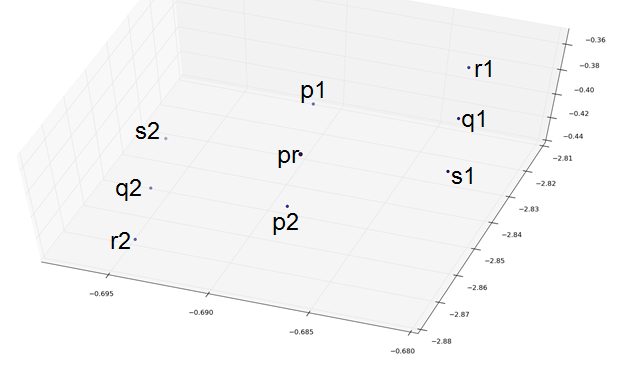
\includegraphics[width=\columnwidth]{figs/dinamica/pontosdinamica.png}
	\caption{Pontos exemplo amostrados da pá.}
	\label{fig::pontosdin}
\end{figure}

%As soluções de cinemática inversa (ângulos das juntas do robô)
%$\Theta_r
%=
%{\theta_{p_r},\theta_{p_1},\theta_{p_2},\theta_{q_1},\theta_{q_2},\theta_{r_1},\theta_{r_2},\theta_{s_1},\theta_{s_2}}$
As velocidades angulares das juntas são calculadas a partir da cinemática
diferencial. Para isso, usa-se o cálculo da matriz jacobiana ($J$), que é a
diferenciação (derivadas parciais) da matriz de cinemática direta em função das
variáveis de junta \citep{sciavicco2000differential}. A velocidade linear do
efetuador ($\dot{X}$) e o jacobiano são conhecidos em cada ponto de referência, logo
podem-se calcular as velocidades das juntas do manipulador entre o ponto de
referência e cada ponto auxiliar: $\dot{X} = J\dot{q}\Rightarrow
J^+\dot{X}=\dot{q}$, onde $J^+$ é a pseudo inversa Moore-Penrose de $J$.

As velocidades angulares são $\Omega_r
=
\{\omega_{p_r,p_1},\omega_{p_r,p_2},\omega_{p_r,q_1},\omega_{p_r,q_2},\omega_{p_r,r_1},\omega_{p_r,r_2},\omega_{p_r,s_1},\omega_{p_r,s_2}\}$,
onde $\omega$, $\omega\in\Omega_r$, é um vetor $n \times 1$, e $n$ é o número de
juntas do robô. As velocidades dos ângulos das juntas é uma informação importate para a
verificação da viabilidade das trajetórias do robô. Para o caso do robô
MH12, onde $\omega_{\textbf{max}}=\{220, 200, 220, 410, 410, 610\}^o/s$, por
exemplo, caso não haja $\omega\in\Omega_r$, tal que
$\omega\leq\omega_{\textbf{max}}$, não é possível realizar o revestimento do
ponto de referência $p_r$. Se $\exists \omega\in\Omega_r$ tal que
$\omega\leq\omega_{\textbf{max}}$, o ponto de referência é viável pela
cinemática inversa e pela cinemática diferencial, mas pode ser inviável ainda
pela análise dinâmica, que considera as acelerações, massas e forças do
conjunto.

As equações dinâmicas de um manipulador são também abordados em
\cite{sciavicco2000differential} e possuem duas abordagens bem conhecidas na
literatura: equações de Newton-Euler e equações de Lagrange. O ambiente OpenRave
utiliza o método de Newton-Euler para computar os torques das juntas (dinâmica
inversa): $\tau = M(q)\alpha + C(q,\omega)\omega + G(q) $, onde $\tau$ é o
vetor de torques das juntas, $M$ matriz de massas e momentos de inércia,
$\alpha$ é acelerações das juntas, $C$ matriz de Coriolis, $\omega$ é as
velocidades das juntas e $G$ o vetor de gravidade.

Para a formação da matriz $M$, é necessária a estimação de parâmetros do
manipulador. A estimação dos parâmetros pode ser realizada de maneira iterativa,
isto é, aplicam-se torques nas juntas e, pela resposta
do manipulador, estima-se a matriz \citep{slotine1988adaptive}; ou pelo CAD do
manipulador, por exemplo, pela utilização da ferramenta SolidWorks. Foi utilizado o método de estimação pelo CAD do
manipulador, visto que os manipuladores ainda estavam em estudo e não foram
adquiridos, além disso houve facilidade de aproximar os parâmetros já que o CAD
fornecido pelo fabricante é bem detalhado. 

A aceleração angular, $\alpha$, é necessária para a computação dos torques,
$\tau$. O método analítico para cálculo da aceleração angular das juntas é
através da derivada da equação da cinemática diferencial:
$\ddot{X}=\dot{q}^TH\dot{q}+J\ddot{q} \Rightarrow
\ddot{q}=J^+(\ddot{X}-\dot{q}^TH\dot{q})$ ou
$\alpha=J^+(a-\omega^TH\omega)$, onde $H$ é a matriz Hessiana, isto é, derivada
parcial da matriz jacobiana $J$ \citep{hourtash2005kinematic}. 

Com a informação dos ângulos, velocidades e acelerações das juntas, momentos
de inércia e massa dos elos, o OpenRave calcula a dinâmica inversa através do
método Newton-Euler, obtendo-se os torques. Para cada ponto de referência, há quatro direções
(trajetórias) possíveis amostradas que o efetuador pode percorrer:
$\{(p_1,p_r,p_2),(q_1,p_r,q_2),(r_1,p_r,r_2),(s_1,p_r,s_2)\}$, logo quatro
ângulos, velocidades e acelerações de juntas, portanto são obtidos quatro
possíveis vetores de torques:
$T=\{\tau_{rp},\tau_{rq},\tau_{rr},\tau_{rs}\}$. E, especificamente para o
caso do manipulador MH12, os valores dos torques devem ser inferiores aos
estabelecidos pelo datasheet:
$\tau_{\textbf{max}}=\{-,-,-,22,22,9.8\}\textbf{Nm}$, logo se $\exists \tau\in
T$, tal que $\tau\leq\tau_{\textbf{max}}$, então há uma trajetória viável.

As figuras~\ref{fig::wgeo}, ~\ref{fig::wcin} e ~\ref{fig::wdin} representam a
evolução das análises do manipulador, de um nível mais simples a um nível mais
complexo de detalhamento, o qual avalia velocidades, acelerações e torques das
juntas do manipulador. Ainda deverá ser executada a análise de manipulabilidade
que avalia o sistema de controle do manipulador. Esta análise é importante para
o planejamento de trajetórias do manipulador e para o cálculo das posições
viáveis da base para uma operação completa.



\begin{figure}[h!]	
	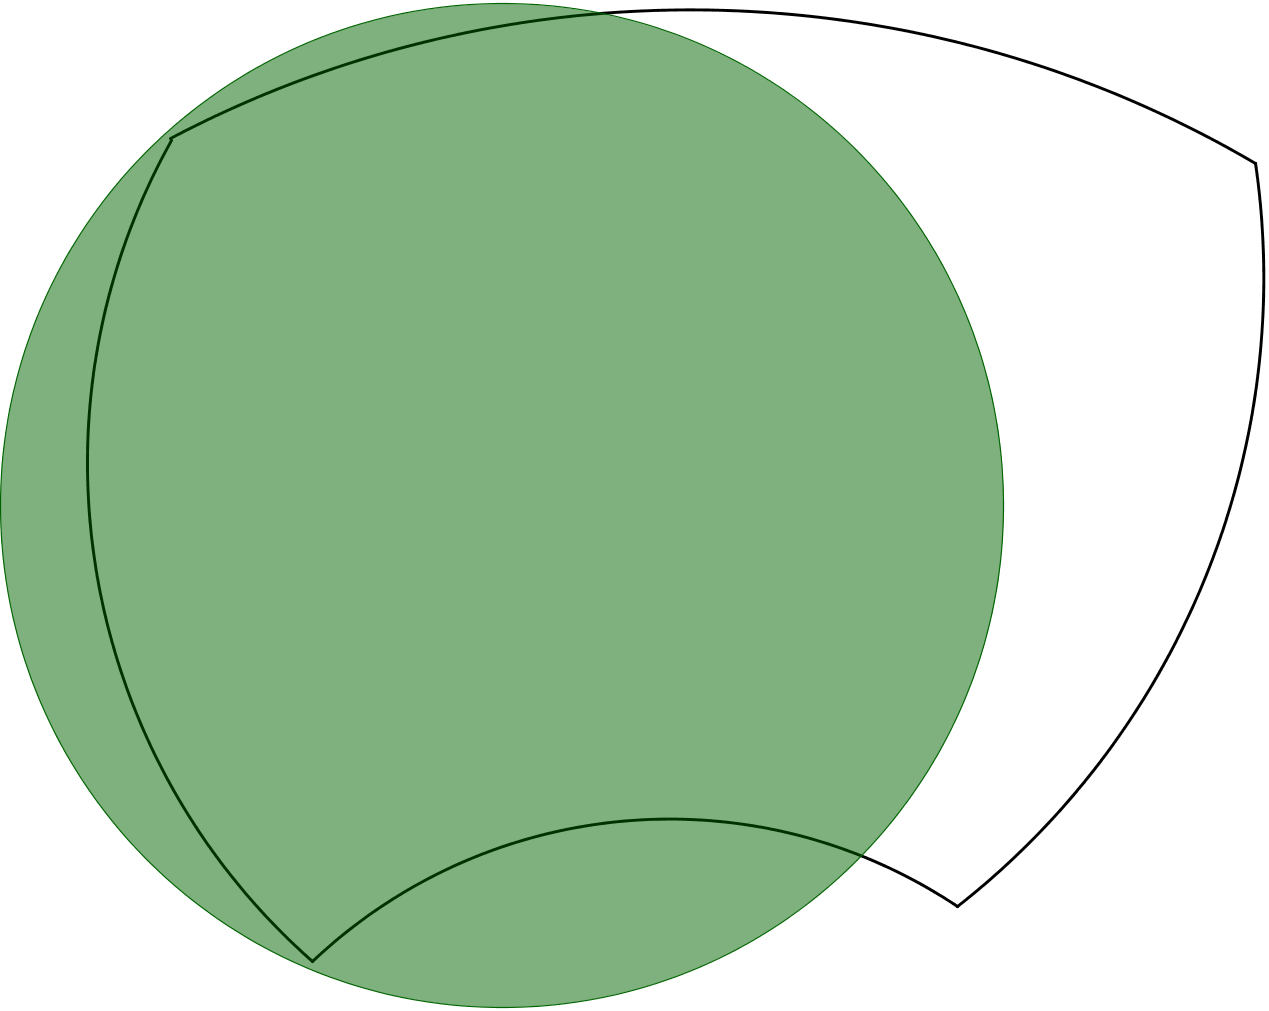
\includegraphics[width=\columnwidth]{figs/dinamica/workspaceGeometrico.png}
	\caption{Área em verde representa a cobertura do revestimento executada pelo
	manipulador, utilizando a abordagem puramente geométrica.}
	\label{fig::wgeo}
\end{figure}

\begin{figure}[h!]	
	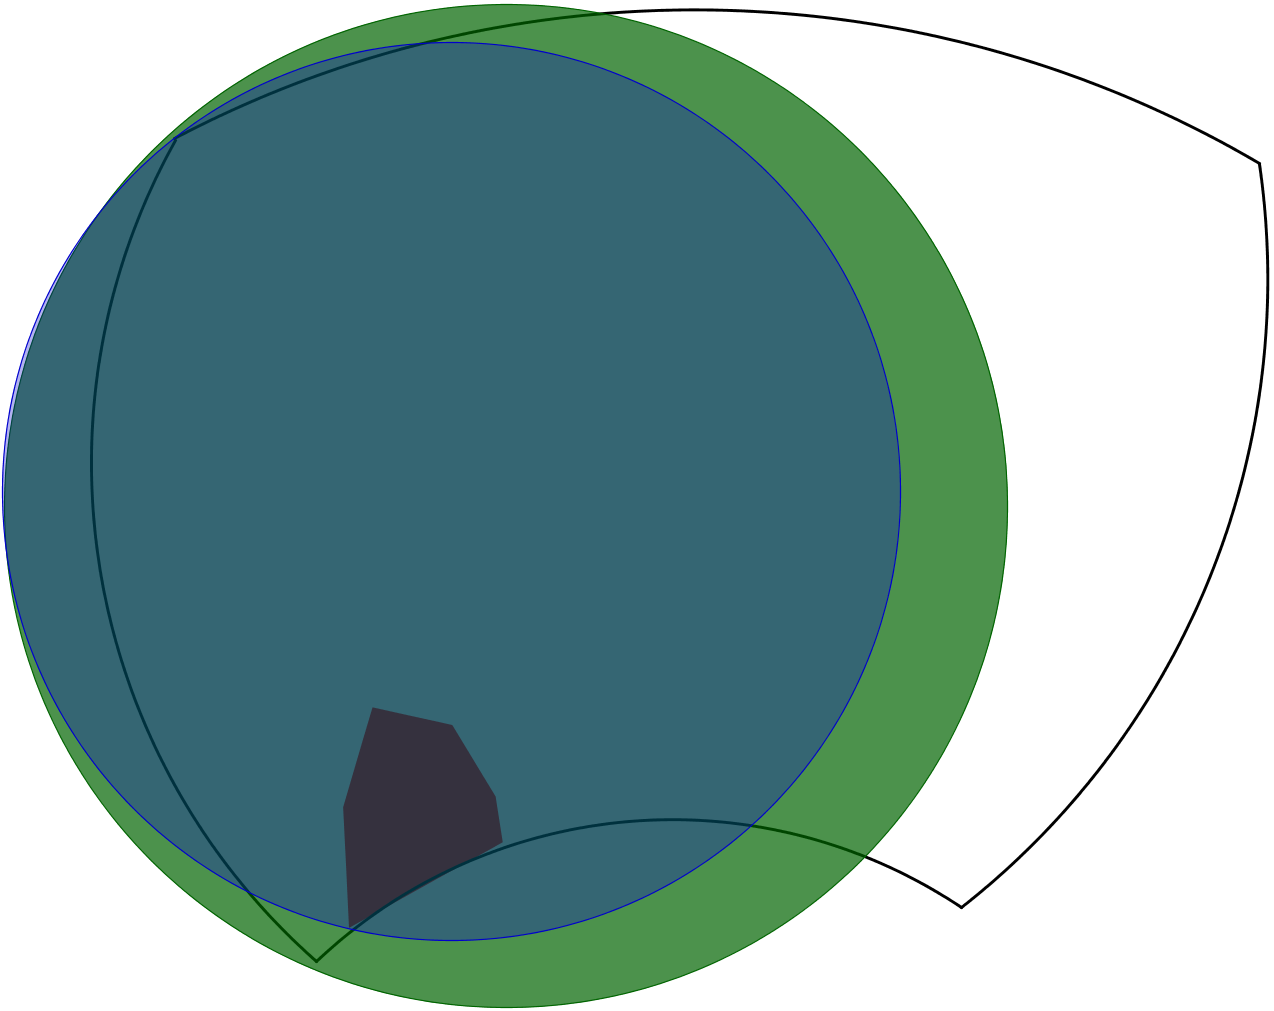
\includegraphics[width=\columnwidth]{figs/dinamica/workspaceCinematica.png}
	\caption{Área em verde representa a cobertura do revestimento executada pelo
	manipulador, utilizando a abordagem puramente cinemática.}
	\label{fig::wcin}
\end{figure}

\begin{figure}[h!]	
	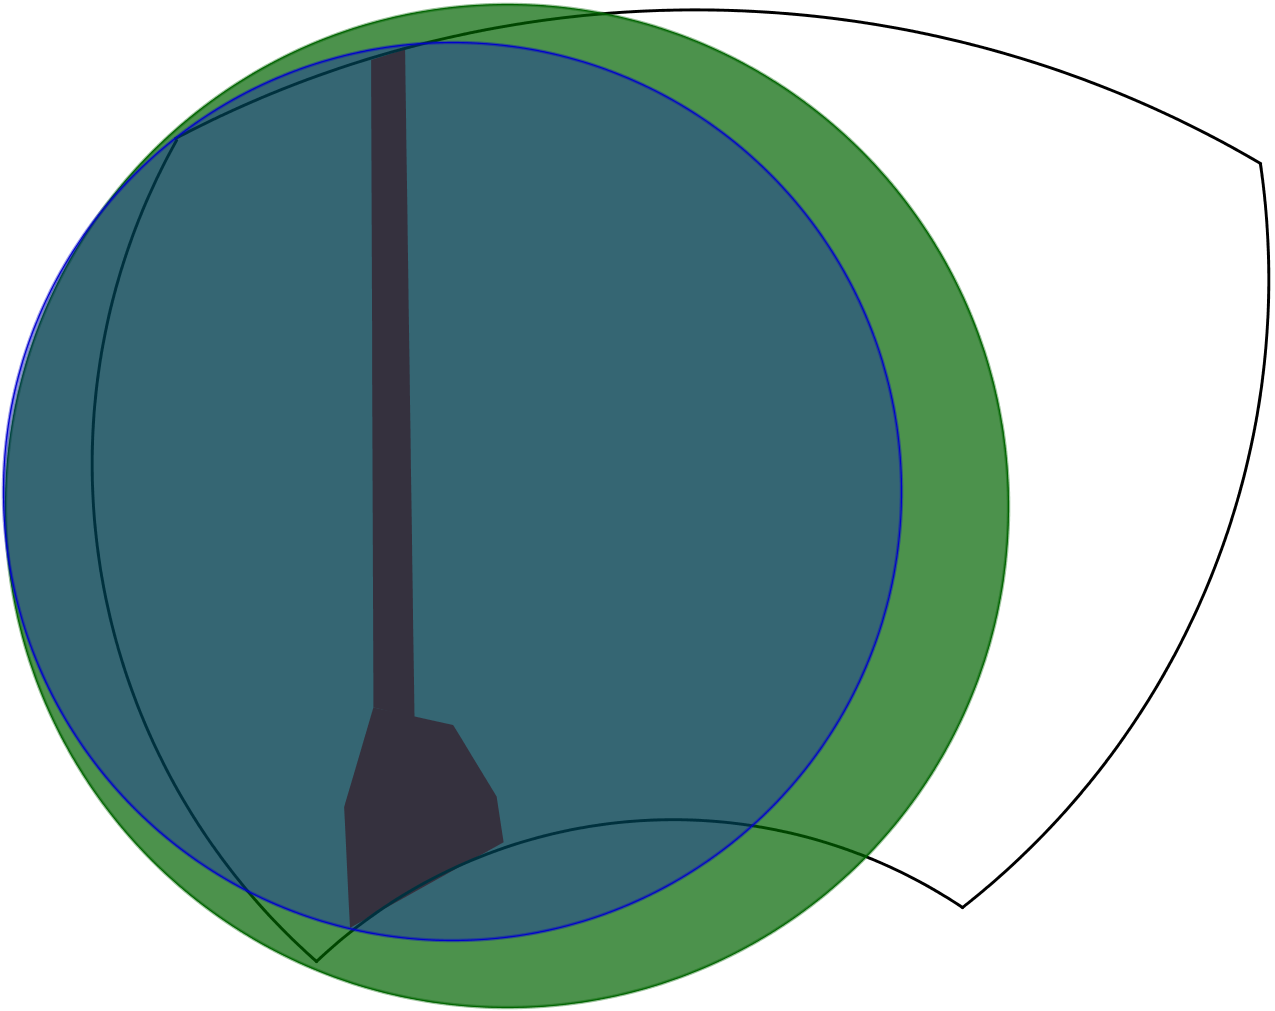
\includegraphics[width=\columnwidth]{figs/dinamica/workspaceTorques.png}
	\caption{Área em verde representa a cobertura do revestimento executada pelo
	manipulador, utilizando a abordagem dinâmica.}
	\label{fig::wdin}
\end{figure}

\subsection{Shutter}%TODO mudar o nome do sistema de desvio do fluxo de
% revestimento
O processo de revestimento HVOF (\textit{High Velocity Oxygen Fuel}) requer
velocidade da pistola controlada de $40~m/min$. Esta velocidade é essencial para
a qualidade do processo e deve ser mantida constante para se obter uma camada 
regular de material ao longo de toda a superfície da peça. Na solução
pesquisada demonstou-se ser inviável utilizar um robô de grande porte, devido a
limitação de acesso e ao confinamento do manipulador no ambiente. Portanto, o
manipulador  escolhido realizará o processo em regiões delimitadas da
superfície da peça e, em sua trajetória, haverá inevitavelmente mudanças de
direção, e portanto acelerações, que irão variar a velocidade da pistola.
Durante essas variações não deve-se injetar o material na peça, sendo necessário um mecanismo
autônomo para impedir o processo nestes intervalos.

A ideia inicialmente estudada foi de uma barreira (\textit{shutter}) ao fluxo na
saída da pistola.
A figura~\ref{fig::shutter_todos} ilustra a ideia para dois conceitos nas
configurações aberta e fechada. 
Nestes conceitos, uma barreira é movimentada automaticamente sempre que houver
mudança de direção da pistola, impedindo que o fluxo de material atinja a
pistola. 

\begin{figure}[h!]
   \centering
   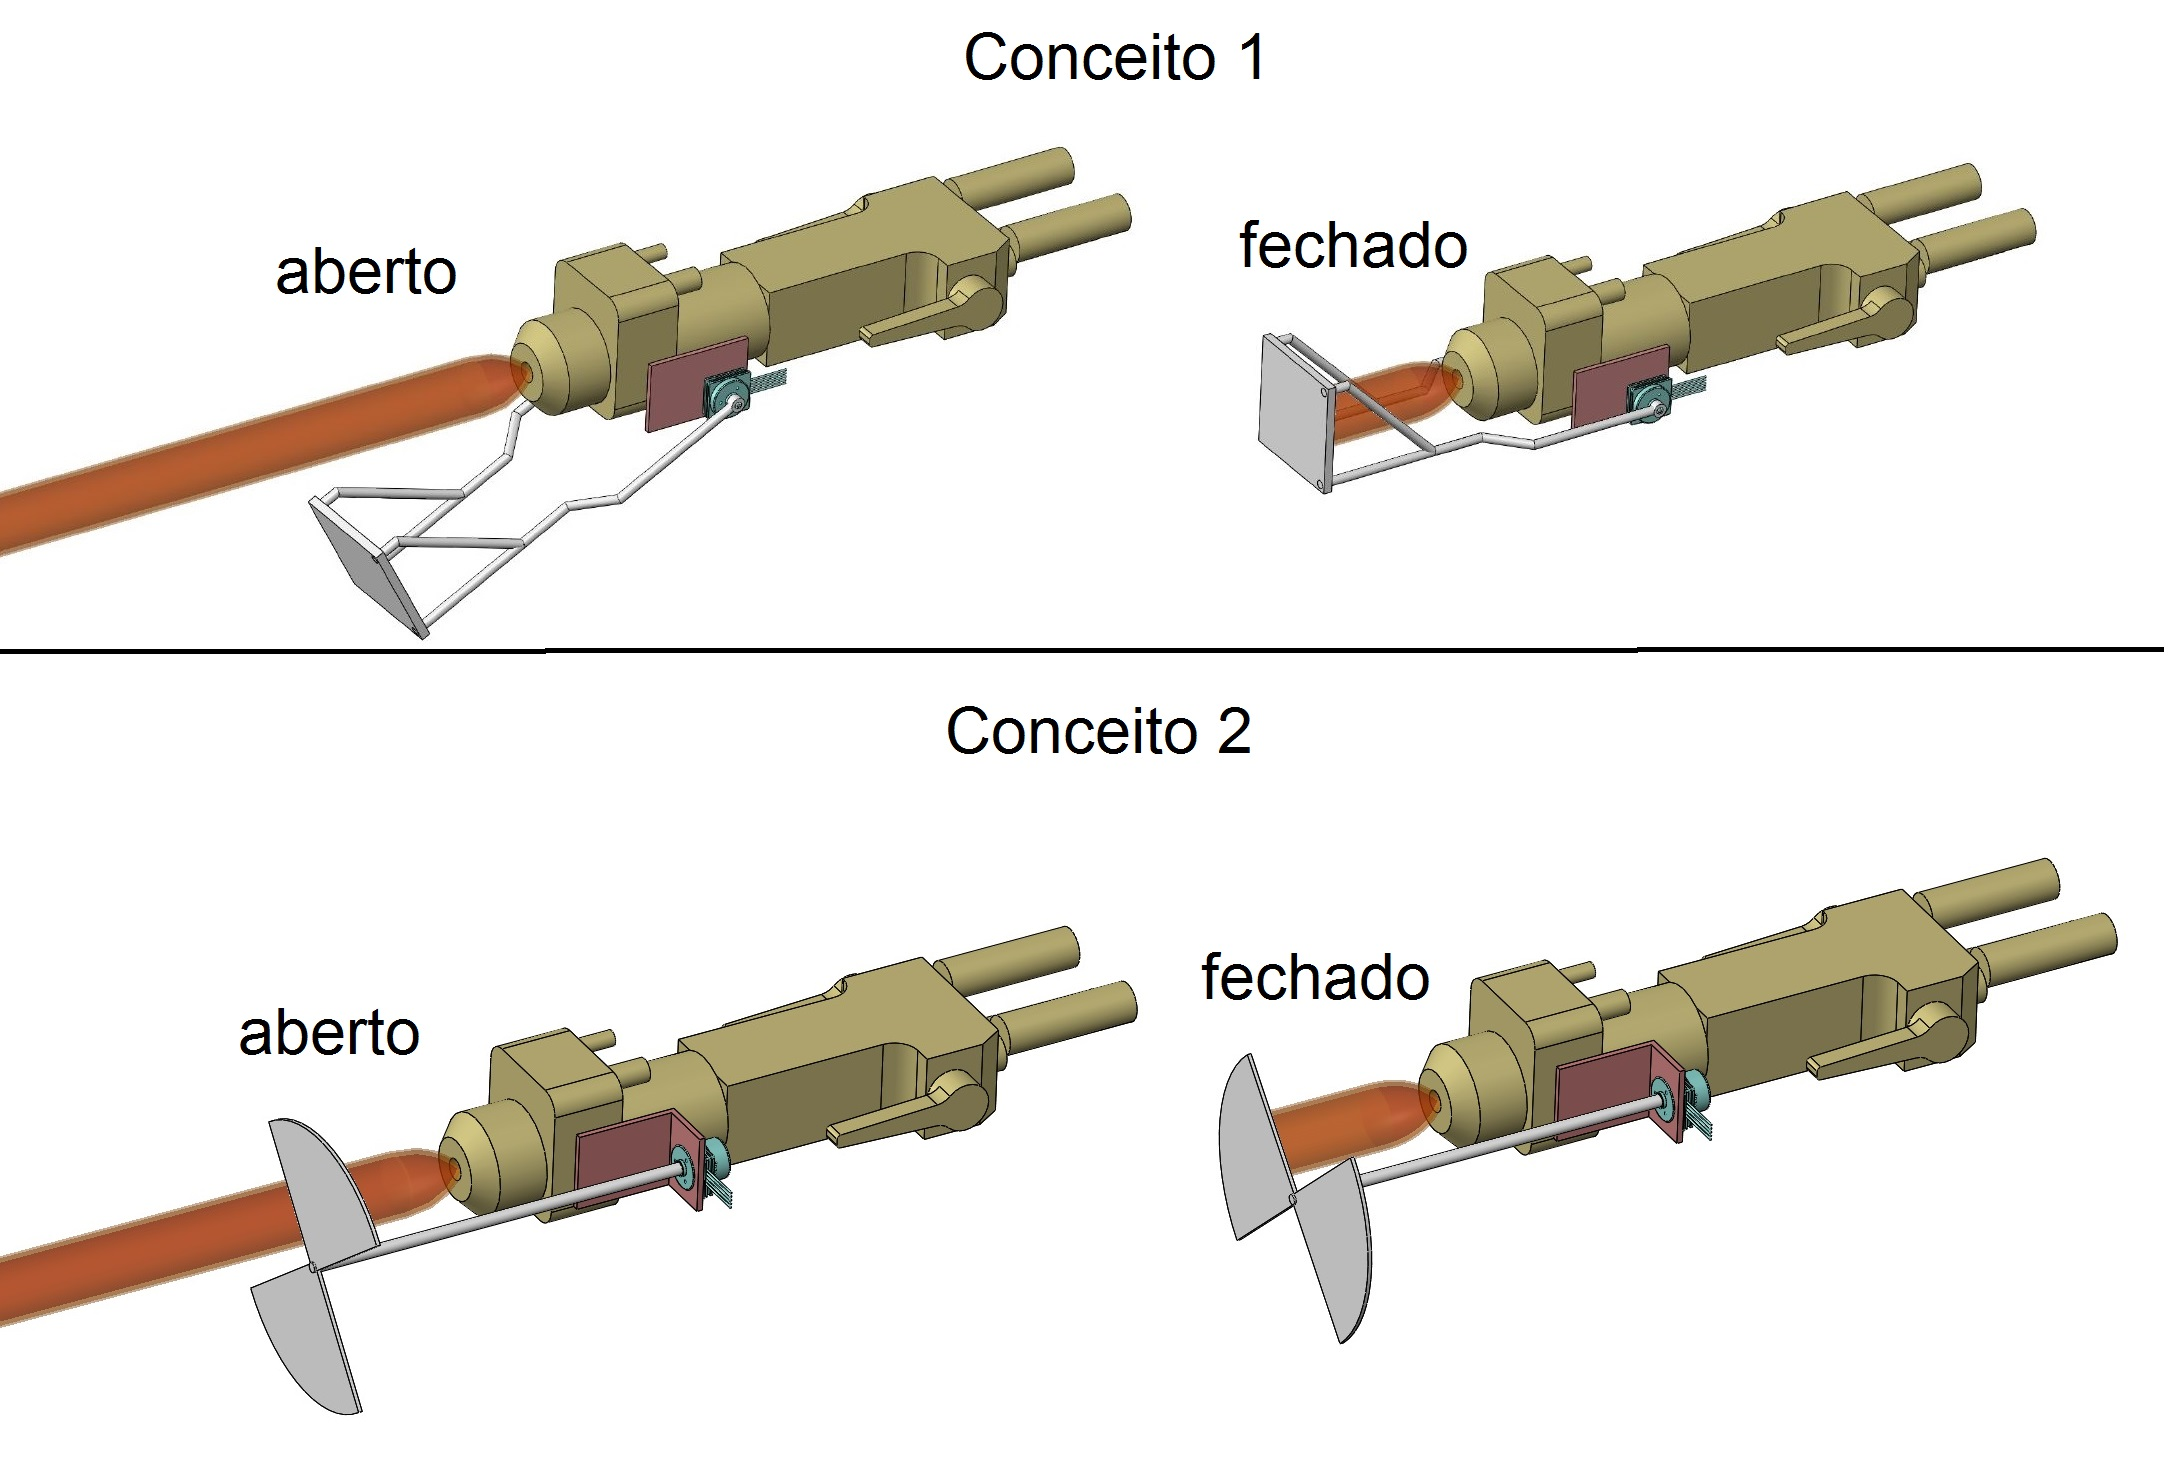
\includegraphics[width=0.8\columnwidth]{figs/shutter/shutter_todos}
   \caption{Conceitos de \textit{shutter} avaliados}
   \label{fig::shutter_todos}
\end{figure}

Algumas considerações foram levantadas para avaliar a viabilidade
desta solução, como a alta temperatura da chama, a capacidade do atuador, a
resistência mecânica da barreira e a taxa de acúmulo de material. Este conceito
foi abandonado principalmente devido ao acúmulo de material na barreira, o que
levaria a um aumento de seu peso, e por consequência momento de inércia,
alterando a dinâmica prevista, ou ainda, poderia chegar a obstruir a saída da
chama causando danos à pistola.

Outra proposta que está sendo estudada é a de modificar o fluxo da linha de
revestimento. A ideia é a inclusão de uma válvula direcional com atuação por
solenóide para desviar o fluxo do material de revestimento para um tanque ou
cilindro de retorno. Esta atuação deve ser autônoma e coordenada com a
trajetória do manipulador. A válvula seria de três vias e duas posições ($3/2$) tal que, no 
repouso, direciona-se o fluxo diretamente para a pistola e, quando
atuada, bloqueia-se o fluxo para a pistola e abre-se o fluxo para exaustão. Uma
válvula limitadora de pressão regulável seria utilizada na linha de exaustão
para igualar as diferenças de pressão entre as duas vias, minimizando efeitos
transitórios.
Outra característica opcional importante para redução dos efeitos transitórios,
como pico de pressão, é a de sobreposição aberta, ou seja, o fluxo só seria
fechado da posição inicial quando o movimento de troca estivesse completo. 
A figura~\ref{fig::circuito_hvof} apresenta o circuito do processo HVOF de forma
simplificada.

 \begin{figure}[h!]
   \centering
   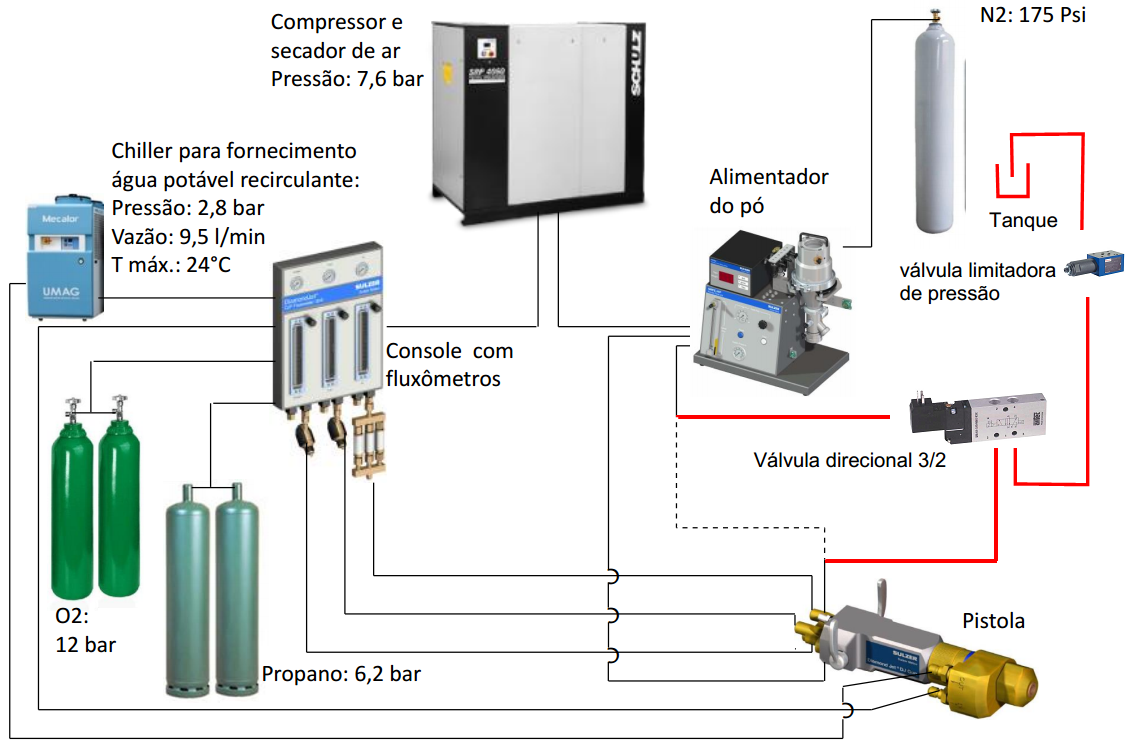
\includegraphics[width=0.8\columnwidth]{figs/shutter/Circuito_HVOF_mod}
   \caption{Circuito do processo HVOF modificado}
   \label{fig::circuito_hvof}
\end{figure}

A linha tracejada representa o circuito original, as linhas em vermelho
representam a modificação do circuito com os equipamentos adicionais indicados.

Esta é uma alternativa que tem como principal vantagem a de poder retornar a
matéria-prima do revestimento para tanque, ou seja, evita-se
o desperdício do material no ambiente. Esta matéria-prima poderia então ser
reaproveitada no processo, separando-se o gás.


\input{conclusao}
  
\bibliography{main} 
\appendix
\end{document}
